\documentclass[12pt]{report}

\usepackage{multirow}
\usepackage{doublespace}
\usepackage{csmthesis}
\usepackage{aaai-bib}
\usepackage[round,authoryear]{natbib} % for citation style

%Place content-specific packages
\usepackage{times}
\usepackage{helvet}
\usepackage{courier}
%\usepackage{epsfig}
\usepackage{graphicx}
%\usepackage{subfigure}

%removing this because this template defines \comment{} as a command
%\usepackage{verbatim} % for comment environment

%\usepackage{array} % for table m attribute
\usepackage{amsmath} % for split, align in equation env and text in math env
\usepackage{caption}
%\usepackage{xspace}
%\usepackage[leqno]{amsmath}
%\usepackage{amssymb}
%\usepackage{dsfont}

%\bibliographystyle{mlapa}

\usepackage{geometry}
%\geometry{verbose, letterpaper, dvips, tmargin=1in, lmargin=1.6in, rmargin=0.9in, bmargin=1in, total={6in,9in}, includeheadfoot, headsep=12pt}
\geometry{verbose, letterpaper, dvips, tmargin=1in, lmargin=1.6in, rmargin=0.9in, bmargin=1in, total={6in,9in}, headsep=12pt}

\usepackage{algpseudocode}  % for algorithm formatting
\usepackage{algorithm}   % for algorithm formatting

\usepackage{amsthm} %for theorem and proof env command
\usepackage{amsfonts} % for integer set symbol and mathcal
\usepackage{url} %bib file uses \url
\usepackage{array} % for table m attribute
\usepackage{listings} % for lstlisting env

\usepackage{lscape} % for landscape

\newcommand{\etal}{et al.\xspace}
\newcommand{\eg}{e.g.,\xspace}
\newcommand{\comment}[1]{}


\def\newnot#1{\label{#1}}

\def\ni{\noindent}
\newcommand{\header}[1]{\noindent \bf{#1}\rm \\ \ni }
% psfigTeX macros
%
% All software, documentation, and related files in this distribution of
% psfig/tex are Copyright (c) 1987 Trevor J. Darrell
%
% Permission is granted for use and non-profit distribution of psfig/tex 
% providing that this notice be clearly maintained, but the right to
% distribute any portion of psfig/tex for profit or as part of any commercial
% product is specifically reserved for the author.
%
% Psfig/tex version 1.1
%
% file last modified: $Header: /home/group-folders/segmentation/cvsroot//devina/peruse/thesis/psfig.tex,v 1.1.1.1 2002/11/04 17:07:44 devina Exp $
%
\catcode`\@=11\relax
\newwrite\@unused
\def\typeout#1{{\let\protect\string\immediate\write\@unused{#1}}}
\typeout{psfig: version 1.1}
\def\psglobal#1{
\typeout{psfig: including #1 globally}
\immediate\special{ps:plotfile #1 global}}
\def\psfiginit{\typeout{psfiginit}
\immediate\psglobal{/usr/lib/ps/figtex.pro}}
%
% @psdo control structure -- similar to Latex @for.
% I redefined these with different names so that psfig can
% be used with TeX as well as LaTeX, and so that it will not 
% be vunerable to future changes in LaTeX's internal
% control structure,
%
\def\@nnil{\@nil}
\def\@empty{}
\def\@psdonoop#1\@@#2#3{}
\def\@psdo#1:=#2\do#3{\edef\@psdotmp{#2}\ifx\@psdotmp\@empty \else
    \expandafter\@psdoloop#2,\@nil,\@nil\@@#1{#3}\fi}
\def\@psdoloop#1,#2,#3\@@#4#5{\def#4{#1}\ifx #4\@nnil \else
       #5\def#4{#2}\ifx #4\@nnil \else#5\@ipsdoloop #3\@@#4{#5}\fi\fi}
\def\@ipsdoloop#1,#2\@@#3#4{\def#3{#1}\ifx #3\@nnil 
       \let\@nextwhile=\@psdonoop \else
      #4\relax\let\@nextwhile=\@ipsdoloop\fi\@nextwhile#2\@@#3{#4}}
\def\@tpsdo#1:=#2\do#3{\xdef\@psdotmp{#2}\ifx\@psdotmp\@empty \else
    \@tpsdoloop#2\@nil\@nil\@@#1{#3}\fi}
\def\@tpsdoloop#1#2\@@#3#4{\def#3{#1}\ifx #3\@nnil 
       \let\@nextwhile=\@psdonoop \else
      #4\relax\let\@nextwhile=\@tpsdoloop\fi\@nextwhile#2\@@#3{#4}}
% 
%
\def\psdraft{
	\def\@psdraft{0}
	%\typeout{draft level now is \@psdraft \space . }
}
\def\psfull{
	\def\@psdraft{100}
	%\typeout{draft level now is \@psdraft \space . }
}
\psfull
\newif\if@prologfile
\newif\if@postlogfile
%%% These are for the option list.
%%% A specification of the form a = b maps to calling \@p@@sa{b}
\newif\if@bbllx
\newif\if@bblly
\newif\if@bburx
\newif\if@bbury
\newif\if@height
\newif\if@width
\newif\if@rheight
\newif\if@rwidth
\newif\if@clip
\def\@p@@sclip#1{\@cliptrue}
\def\@p@@sfile#1{%\typeout{file is #1}
		   \def\@p@sfile{#1}
}
\def\@p@@sfigure#1{\def\@p@sfile{#1}}
\def\@p@@sbbllx#1{
		%\typeout{bbllx is #1}
		\@bbllxtrue
		\dimen100=#1
		\edef\@p@sbbllx{\number\dimen100}
}
\def\@p@@sbblly#1{
		%\typeout{bblly is #1}
		\@bbllytrue
		\dimen100=#1
		\edef\@p@sbblly{\number\dimen100}
}
\def\@p@@sbburx#1{
		%\typeout{bburx is #1}
		\@bburxtrue
		\dimen100=#1
		\edef\@p@sbburx{\number\dimen100}
}
\def\@p@@sbbury#1{
		%\typeout{bbury is #1}
		\@bburytrue
		\dimen100=#1
		\edef\@p@sbbury{\number\dimen100}
}
\def\@p@@sheight#1{
		\@heighttrue
		\dimen100=#1
   		\edef\@p@sheight{\number\dimen100}
		%\typeout{Height is \@p@sheight}
}
\def\@p@@swidth#1{
		%\typeout{Width is #1}
		\@widthtrue
		\dimen100=#1
		\edef\@p@swidth{\number\dimen100}
}
\def\@p@@srheight#1{
		%\typeout{Reserved height is #1}
		\@rheighttrue
		\dimen100=#1
		\edef\@p@srheight{\number\dimen100}
}
\def\@p@@srwidth#1{
		%\typeout{Reserved width is #1}
		\@rwidthtrue
		\dimen100=#1
		\edef\@p@srwidth{\number\dimen100}
}
\def\@p@@sprolog#1{\@prologfiletrue\def\@prologfileval{#1}}
\def\@p@@spostlog#1{\@postlogfiletrue\def\@postlogfileval{#1}}
\def\@cs@name#1{\csname #1\endcsname}
\def\@setparms#1=#2,{\@cs@name{@p@@s#1}{#2}}
%
% initialize the defaults (size the size of the figure)
%
\def\ps@init@parms{
		\@bbllxfalse \@bbllyfalse
		\@bburxfalse \@bburyfalse
		\@heightfalse \@widthfalse
		\@rheightfalse \@rwidthfalse
		\def\@p@sbbllx{}\def\@p@sbblly{}
		\def\@p@sbburx{}\def\@p@sbbury{}
		\def\@p@sheight{}\def\@p@swidth{}
		\def\@p@srheight{}\def\@p@srwidth{}
		\def\@p@sfile{}
		\def\@p@scost{10}
		\def\@sc{}
		\@prologfilefalse
		\@postlogfilefalse
		\@clipfalse
}
%
% Go through the options setting things up.
%
\def\parse@ps@parms#1{
	 	\@psdo\@psfiga:=#1\do
		   {\expandafter\@setparms\@psfiga,}}
%
% Compute bb height and width
%
\newif\ifno@bb
\newif\ifnot@eof
\newread\ps@stream
\def\bb@missing{
	\typeout{psfig: searching \@p@sfile \space  for bounding box}
	\openin\ps@stream=\@p@sfile
	\no@bbtrue
	\not@eoftrue
	\catcode`\%=12
	\loop
		\read\ps@stream to \line@in
		\global\toks200=\expandafter{\line@in}
		\ifeof\ps@stream \not@eoffalse \fi
		%\typeout{ looking at :: \the\toks200 }
		\@bbtest{\toks200}
		\if@bbmatch\not@eoffalse\expandafter\bb@cull\the\toks200\fi
	\ifnot@eof \repeat
	\catcode`\%=14
}	
\catcode`\%=12
\newif\if@bbmatch
\def\@bbtest#1{\expandafter\@a@\the#1%%BoundingBox:\@bbtest\@a@}
\long\def\@a@#1%%BoundingBox:#2#3\@a@{\ifx\@bbtest#2\@bbmatchfalse\else\@bbmatchtrue\fi}
\long\def\bb@cull#1 #2 #3 #4 #5 {
	\dimen100=#2 bp\edef\@p@sbbllx{\number\dimen100}
	\dimen100=#3 bp\edef\@p@sbblly{\number\dimen100}
	\dimen100=#4 bp\edef\@p@sbburx{\number\dimen100}
	\dimen100=#5 bp\edef\@p@sbbury{\number\dimen100}
	\no@bbfalse
}
\catcode`\%=14
%
\def\compute@bb{
		\no@bbfalse
		\if@bbllx \else \no@bbtrue \fi
		\if@bblly \else \no@bbtrue \fi
		\if@bburx \else \no@bbtrue \fi
		\if@bbury \else \no@bbtrue \fi
		\ifno@bb \bb@missing \fi
		\ifno@bb \typeout{FATAL ERROR: no bb supplied or found}
			\no-bb-error
		\fi
		%
		\count203=\@p@sbburx
		\count204=\@p@sbbury
		\advance\count203 by -\@p@sbbllx
		\advance\count204 by -\@p@sbblly
		\edef\@bbw{\number\count203}
		\edef\@bbh{\number\count204}
		%\typeout{ bbh = \@bbh, bbw = \@bbw }
}
%
% \in@hundreds performs #1 * (#2 / #3) correct to the hundreds,
%	then leaves the result in @result
%
\def\in@hundreds#1#2#3{\count240=#2 \count241=#3
		     \count100=\count240	% 100 is first digit #2/#3
		     \divide\count100 by \count241
		     \count101=\count100
		     \multiply\count101 by \count241
		     \advance\count240 by -\count101
		     \multiply\count240 by 10
		     \count101=\count240	%101 is second digit of #2/#3
		     \divide\count101 by \count241
		     \count102=\count101
		     \multiply\count102 by \count241
		     \advance\count240 by -\count102
		     \multiply\count240 by 10
		     \count102=\count240	% 102 is the third digit
		     \divide\count102 by \count241
		     \count200=#1\count205=0
		     \count201=\count200
			\multiply\count201 by \count100
		 	\advance\count205 by \count201
		     \count201=\count200
			\divide\count201 by 10
			\multiply\count201 by \count101
			\advance\count205 by \count201
			%
		     \count201=\count200
			\divide\count201 by 100
			\multiply\count201 by \count102
			\advance\count205 by \count201
			%
		     \edef\@result{\number\count205}
}
\def\compute@wfromh{
		% computing : width = height * (bbw / bbh)
		\in@hundreds{\@p@sheight}{\@bbw}{\@bbh}
		%\typeout{ \@p@sheight * \@bbw / \@bbh, = \@result }
		\edef\@p@swidth{\@result}
		%\typeout{w from h: width is \@p@swidth}
}
\def\compute@hfromw{
		% computing : height = width * (bbh / bbw)
		\in@hundreds{\@p@swidth}{\@bbh}{\@bbw}
		%\typeout{ \@p@swidth * \@bbh / \@bbw = \@result }
		\edef\@p@sheight{\@result}
		%\typeout{h from w : height is \@p@sheight}
}
\def\compute@handw{
		\if@height 
			\if@width
			\else
				\compute@wfromh
			\fi
		\else 
			\if@width
				\compute@hfromw
			\else
				\edef\@p@sheight{\@bbh}
				\edef\@p@swidth{\@bbw}
			\fi
		\fi
}
\def\compute@resv{
		\if@rheight \else \edef\@p@srheight{\@p@sheight} \fi
		\if@rwidth \else \edef\@p@srwidth{\@p@swidth} \fi
}
%		
% Compute any missing values
\def\compute@sizes{
	\compute@bb
	\compute@handw
	\compute@resv
}
%
% \psfig
% usage : \psfig{file=, height=, width=, bbllx=, bblly=, bburx=, bbury=,
%			rheight=, rwidth=, clip=}
%
% "clip=" is a switch and takes no value, but the `=' must be preset.
\def\psfig#1{\vbox {
	% do a zero width hard space so that a single
	% \psfig in a centering enviornment will behave nicely
	%{\setbox0=\hbox{\ }\ \hskip-\wd0}
	%
	\ps@init@parms
	\parse@ps@parms{#1}
	\compute@sizes
	%
	\ifnum\@p@scost<\@psdraft{
		\typeout{psfig: including \@p@sfile \space }
		%
		\special{ps::[begin] 	\@p@swidth \space \@p@sheight \space
				\@p@sbbllx \space \@p@sbblly \space
				\@p@sbburx \space \@p@sbbury \space
				startTexFig \space }
		\if@clip{
			\typeout{(clip)}
			\special{ps:: \@p@sbbllx \space \@p@sbblly \space
				\@p@sbburx \space \@p@sbbury \space
				doclip \space }
		}\fi
		\if@prologfile
		    \special{ps: plotfile \@prologfileval \space } \fi
		\special{ps: plotfile \@p@sfile \space }
		\if@postlogfile
		    \special{ps: plotfile \@postlogfileval \space } \fi
		\special{ps::[end] endTexFig \space }
		% Create the vbox to reserve the space for the figure
		\vbox to \@p@srheight true sp{
			\hbox to \@p@srwidth true sp{
				\hfil
			}
		\vfil
		}
	}\else{
		% draft figure, just reserve the space and print the
		% path name.
		\vbox to \@p@srheight true sp{
		\vss
			\hbox to \@p@srwidth true sp{
				\hss
				\@p@sfile
				\hss
			}
		\vss
		}
	}\fi
}}
\catcode`\@=12\relax




%%Items repeated throughout the thesis
%\newcommand{\thesistitle}{Rapid Adaptation in Real-time Systems through Solution Space Analysis}
\newcommand{\thesistitle}{Rapid Plan Adaptation Through Offline Analysis of Potential Plan Disruptors}
\newcommand{\fullname}{Robert H. Holder, III}

\renewcommand{\algorithmiccomment}[1]{// #1}

\begin{document}
\title{{\bf \thesistitle{}}}
\author{\fullname{}}
\tolerance=1000
\newpage
\thispagestyle{empty}
\mbox{}

\newpage
\begin{titlepage}
\vspace{0.6in}
\begin{singlespace}

\begin{center}
\vspace{0.1in}
\large{\bf APPROVAL SHEET}
\bigskip \bigskip
\end{center}

\begin{flushleft}
{\bf Title of Thesis:}{\hspace{3mm}}\thesistitle{}\\
\vspace{0.5in}
{\bf Name of Candidate:}{\hspace{3mm}} \parbox[t]{2in}{\fullname{} \\ Ph.D. in Computer Science, 2016}
\end{flushleft}

\vspace{0.5in}

\begin{flushleft}
{\bf Thesis and Abstract Approved:}{\hspace{3mm}} 
\parbox[t]{2.5in}{\underline{\hspace{2.0in}}\\ 
	Dr. Marie desJardins \\
	Professor \\
	Department of Computer Science and \\
	Electrical Engineering}
\end{flushleft}

\vspace{0.5in}

\begin{flushleft}
{\bf Thesis and Abstract Approved:}{\hspace{3mm}} 
\parbox[t]{2.5in}{\underline{\hspace{2.0in}}\\ 
	Dr. Timothy Finin \\
	Professor \\
	Department of Computer Science and \\
	Electrical Engineering}
\end{flushleft}

\vspace{0.8in}

\begin{flushleft}
{\bf Date Approved: December 9, 2015}{\hspace{3mm}} \underline{\hspace{2.5in}}\\
\end{flushleft}

\end{singlespace}
\end{titlepage}
\par\vfil

\newpage
\begin{titlepage}

\begin{center}
\vspace{0.1in}
\large{\bf Curriculum Vitae}
\bigskip \bigskip
\end{center}

\begin{flushleft}
  {\bf Name:}{\hspace{3mm}}\fullname{}.\\
	{\bf Degree and date to be conferred:}{\hspace{3mm}}Ph.D. in Computer Science, May 2016. \\
	{\bf Collegiate institutions attended:}\\
	\begin{singlespace} 
	{\hspace{0.4in}}University of Maryland Baltimore County, Ph.D. Computer Science, 2016. \\
	{\hspace{0.4in}}\parbox[t]{5.5in}{Tulane University, M.S. Computer Science, 2000.} \\
        {\hspace{0.4in}}\parbox[t]{5.5in}{Tulane University, B.S. Computer Science, 1999.} \\
	\end{singlespace} 
	\vspace{8pt}
	{\bf Professional publications:}\\
	\begin{singlespace} 
{\hspace{0.4in}} \parbox[t]{5.5in}{B. Bauer, D. Scheidt, P. Rosendall, N. Rolander, \textbf{R. Holder}, E. Schmidt, and F. Ferrese.  ``Evaluating Test Methods for a Complex Connected System.''  American Institute of Aeronautics and Astronautics, March 2011.}\\
{\vspace{5pt}}

{\hspace{0.4in}} \parbox[t]{5.5in}{\textbf{R. Holder}.  ``Problem Space Analysis for Plan Library Generation and Algorithm Selection in
Real-time Systems.'' In Proceedings of The 23rd International FLAIRS Conference, May 2010, Daytona Beach, FL.  \textbf{Best Poster Award.}}\\
{\vspace{5pt}}

{\hspace{0.4in}} \parbox[t]{5.5in}{\textbf{R. Holder} and R.S. Cost.  ``Utilizing Resource Brokering Within Virtual Environments to Support Distributed Collaboration and Rapid Team Configuration.'' Proceedings of the 14th ICCRTS, June 2009, Washington, D.C.}\\
{\vspace{5pt}}

{\hspace{0.4in}} \parbox[t]{5.5in}{\textbf{R. Holder} and R.S. Cost.  ``Challenges of Resource Integration for C2 Collaborations within Virtual Environments.''  Proceedings of 2008 Proteus Futures Academic Workshop, Sept 2008, Carlisle, PA.}
\end{singlespace} 

\vspace{8pt}
	{\bf Professional positions held:}\\
	\begin{singlespace}
	{\hspace{0.4in}}\parbox[t]{5.5in}{Computer Scientist, Johns Hopkins University Applied Physics Laboratory (August 2000 -- December 2014).}\\
	{\hspace{0.4in}}\parbox[t]{5.5in}{Senior Software Engineer, ClearEdge IT Solutions, LLC (January 2015 -- Current).}\\	\end{singlespace}
\end{flushleft}
       
\end{titlepage}
\par\vfil



\newpage
\newpage
\pagestyle{empty}

\begin{center}
\vspace{0.1in}
\large{\bf ABSTRACT} \par  
\bigskip \bigskip
\end{center}

\begin{flushleft}
{\bf Title of Thesis:} \thesistitle{}\\
\fullname{}, Ph.D. in Computer Science, 2016 \\
\begin{singlespace}
{\bf Thesis directed by:}{\hspace{2.5mm}} \parbox[t]{3in}{Dr. Marie desJardins, Professor and \\ Dr. Tim Finin, Professor \\
Department of Computer Science and \\ Electrical Engineering}
\end{singlespace}
\end{flushleft}


Computing solutions to intractable planning problems is particularly problematic in dynamic, real-time domains.  For example, visitation planning problems, such as a delivery truck that must deliver packages to various locations, can be mapped to a Traveling Salesman Problem (TSP).  The TSP is an NP-complete problem, requiring planners to use heuristics to find solutions to any significantly large problem instance, and can require a significant amount of time.  Planners that solve the dynamic variant, the Dynamic Traveling Salesman Problem (DTSP), calculate an efficient route to visit a set of potentially changing locations \citep{psaraftis88dynamic}.  When a new location becomes known, DTSP planners typically use heuristics to add the new locations to the previously computed route.  Depending on the placement and quantity of these new locations, the efficiency of this adapted, approximated solution can vary significantly \citep{psaraftis95dynamic,laporte00classical,larsen2000dvrp}.  Solving a DTSP in real time thus requires choosing between a TSP planner, which produces a relatively good but slowly generated solution, and a DTSP planner, which produces a less optimal solution relatively quickly.

Instead of quickly generating approximate solutions or slowly generating better solutions at runtime, this dissertation introduces an alternate approach of precomputing a library of high-quality solutions \textit{prior} to runtime.  One could imagine a library containing a high-quality solution for every potential problem instance consisting of potential new locations, but this approach obviously does not scale with increasing problem complexity.  Because complex domains preclude creating a comprehensive library, I instead choose a subset of all possible plans to include. Strategic plan selection will ensure that the library contains appropriate plans for future scenarios.

Experimental results demonstrate that plan quality comparable to online repair can be achieved by calculating solutions for a sample of the potential problem instances.  I present novel algorithms that use the sampled solutions to find approximate solutions to other problem instances by exploiting structure in the solution space.  For domains with solution spaces that do not contain sufficient structure, I show that applying abstraction, normalization, and reindexing operations to the solutions can create the necessary structure.  For the domains tested, the algorithms generated full plan libraries containing solutions as good or better than online repair by calculating solutions to as few as 0.2\% of the potential problem instances.

This dissertation thus contributes (1) a representation framework to reason about the structure of solution spaces, (2) novel algorithms to exploit structure in the solution space in order to generate plan libraries, (3) techniques to transform the structure of the solution space to facilitate the use of the algorithms, and (4) an evaluation of the algorithms in several test domains.


%Properly indexed, problem instances with the same solutions tend to be clustered in homogeneous regions within the problem space. The algorithms presented in this dissertation attempt to discover these regions by sampling the problem space, and estimate the overall structure of the space. 
%There are a large number of new problem instances, but generally a much smaller number of unique plans
%Thus the strategy is to identify the clusters



% Be certain to add one final blank page to the thesis when you submit it (according to 2005 UMBC Grad School Formatting Requirements).  The template does not do this automatically so that the table of contents won't include a blank entry.

\par\vfil


\newpage
\begin{titlepage}
\mbox{}\vspace{1in}
\begin{center}

    {\Large \bf \thesistitle{} \par}
    
\vspace{2in}

    {\large by} \\
    {\large \fullname{}}
    
\vspace{2in}

  \begin{singlespace}
    Thesis submitted to the Faculty of the Graduate School \\
    of the University of Maryland in partial fulfillment \\
    of the requirements for the degree of \\
    Doctor of Philosophy in Computer Science \\
    2015
	\end{singlespace}
\end{center}
\end{titlepage}

\newpage
\begin{titlepage}
\mbox{}\vspace{7.5in}
\begin{center}
\copyright~Copyright \fullname{} 2016
\end{center}
\end{titlepage}

\newpage
\thispagestyle{empty}
\mbox{}

%\frontmatter
\pagenumbering{roman}

\newpage
\setcounter{page}{2}
\cleardoublepage
\newpage
\newpage
\fchapter[Dedication]{}
\thispagestyle{plain}
%\begin{titlepage}
\vfil\null
\begin{center}

\mbox{}\vspace{3in}

\emph{Dedicated to (soon-to-be-Dr.) Michelle Beadle Holder.}

\end{center} 
\normalsize
\vfil\null
%\end{titlepage}

\cleardoublepage
\fchapter{ACKNOWLEDGMENTS}
\pagestyle{plain}

I would like to thank Dr.~Tim Finin and Dr.~Marie desJardins for their help and patience in helping me complete this process on a part-time basis since 2004.  Appreciation is also extended to my committee, Dr.~Tim Oates, Dr.~Scott Cost, and Dr.~Donald Miner for their feedback and flexibility.

I also would like to thank the PROMISE program, directed by Dr.~Renetta Tull, for the amazing amount of support supplied over the course of completing this degree.

Thanks also are extended to the Johns Hopkins University Applied Physics Laboratory for its support of my continuing education.  Many individuals from the Lab were very supportive in this endeavor.  Rose Daley introduced me to this problem area as part of a DARPA project.  Dr.~I-Jeng Chang, Dr.~Scott Cost, John Piorkowski, Dr.~Ralph Semmel, Dr.~David Silberberg, Dr.~Paul McNamee, and David Watson were some of many individuals who guided me in various ways.

Various fellow graduate students were also instrumental in accomplishing this goal.  In particular, I would like to mention Dr.~Blazej Bulka, Dr.~Eric Eaton, Dr.~James MacGlashan, Dr.~Patti Ord\'{o}\~{n}ez Rozo, and Dr.~Donald Miner.

\cleardoublepage
\tableofcontents
\cleardoublepage
\listoffigures
\cleardoublepage
\listoftables
\cleardoublepage

%\mainmatter
\pagenumbering{arabic}
\pagestyle{myheadings}
\markright{}

\chapter{Introduction \& Motivation}
\thispagestyle{plain}

\label{ch:introduction}

The ability of a planning system to quickly adapt to environmental changes is critical in time-constrained domains.  Online, heuristic plan repair approaches are sufficient for small changes in the environment; however, repeated or large changes can cause plan quality to degrade. I present an approach that uses available offline time to analyze the space of potential changes in the environment and creates a mapping between problem instances and solutions for use during runtime.  I show that this approach allows a system to rapidly adapt to changes, while yielding plan quality that is comparable to traditional online approaches.


The motivation for this work stems from the common theme encountered in the course of my work in several domains including shipboard computing resource management, mine-like object visitation, and mobile sensor scheduling.  The shipboard computing resource management task is to allocate computing resources to critical ship processes to support overall ship function. However, if a negative event impacts the ship, then a significant number of the computing resources can suddenly become unavailable.  In this case, the system must quickly reallocate the remaining computing resources to the critical processes such that overall ship function remains viable.

In the mine-like object (MLO) visitation domain, one or more ships must visit all of the MLOs in a region to determine if the object is actually a mine or some other innocuous artifact.  Ideally, this would be done as quickly as possible in order to certify the region as safe for travel.  During the course of visiting the known MLOs, a new MLO may be detected by a satellite or other means.  In this case, the routes of the ships in the region must be recalculated to incorporate this new location.

The mobile sensor scheduling problem is similar to the MLO domain except that, one, the mobile sensor only has to pass close enough to a location to receive of sample of its broadcasts, and, two, it must sample the broadcasts within one or more time windows.  In this problem, similar to the MLO domain, new locations and time windows can be introduced and must be incorporated into the schedule of each sensor.

In all of these domains, it is useful to maintain a high quality plan, even when the requirements of the problem change.  The range of change typically occurs on a small number of dimensions, and arrives slowly enough such that replanning does not have to take into account a large number of changes.  Thus, the experiments in this domain tend to reflect that bias.  However, future work does discuss how the approaches proposed in the dissertation would scale to larger problems.



\section{Planning}

Planning is the branch of artificial intelligence concerned with efficiently generating sequences of actions, i.e., \textit{plans}, to achieve goals.  Typically, a planning domain consists of a set of states, described by state variables; a set of available actions, described by their effects on state variables; and one or more goal states.  A planning problem defines a starting state, and the task of the planner is to find a set of actions that transform the starting state into a goal state.  Depending on the complexity of the problem, finding any feasible plan may be satisfactory; in other cases, finding the least expensive plan in terms of length or some total action cost is desired.

Planning for environments in which the planner has a limited amount of time to produce a plan is called \textit{time-constrained planning}.  This type of planning applies to situations in which the usefulness, or \textit{utility}, of a plan degrades over time.  Typically, a tradeoff exists between spending more time searching the space for a better plan and quickly deciding on a plan that may have lower utility.  When some prior plan already exists, the planner can either repair the current plan, which is typically faster, or replan, which typically yields better utility.


%For example, consider the classic planning domain of Blocks World.  In this domain the planner must produce one or more stacks of blocks at a one or more specific locations from a set of blocks scattered or stacked on a table.  The planner is allowed to move a block to a location on the table or on top of another block.  Thus a state consists of the location of each of the blocks.  Actions might be defined such as ``move-block \textit{block} onto \textit{object}'' with the precondition that the block does not have another object on top of it, or is \textit{clear}.  Additionally, the object must either be the table or a distinct block that is clear.

I will use the traveling salesman problem (TSP) planning problem as a reference problem throughout much of this dissertation.  The TSP requires a solver to find the shortest route that visits a given set of locations.  This is a classic NP-complete problem that has been studied widely in computer science.  In the basic problem, all of the locations are static.  The dynamic variant, the DTSP, allows locations to be introduced to the planner after execution begins.


\section{Overview of Problem Space Approximation}

Instead of computing approximate solutions at runtime, my approach is to precompute a library of high-quality solutions \textit{prior} to runtime.  In the case of DTSP, one could imagine a library containing a high-quality\footnote{``High-quality'' refers to the plan generated by an offline heuristic solver.  Since a heuristic solver creates an approximate solution, the result cannot be assumed to be optimal.  Thus, I describe the resulting solutions as ``high-quality'' rather than optimal, ideal, or exact.} solution for every possible combination of potential new destinations.  Obviously, as the scale of the planning problem increases, the level of complexity precludes creating a comprehensive library, so in practice a library can only contain a subset of all possible plans. Therefore, I also introduce methods to ensure that the library contains appropriate plans for use when the planning environment changes.

An understanding of the problem space characteristics can be used to choose the planning scenarios for which to generate solutions.  In particular, identifying regions of problem instances with identical solutions allows for the efficient creation of a mapping from problem instances to solutions, called a \textit{Problem-Solution Map} (PS Map).  A PS Map is a component of \textit{problem space analysis} (PSA), which allows a system to make informed decisions about which solutions to include in the library.

Problem instances contain characteristics that are identical, called \textit{static characteristics}, and characteristics that differ between them, the \textit{variable features}, that lead to differences in the problem instance solutions.  The PS Map represents a library of solutions for problem instances, indexed by the variable features of the set of problem instances.  This map provides a mapping from a problem instance to its solution, showing the changes in the solutions as a function of the variable features within the problem instances.  I will discuss several techniques to efficiently build this map.

\section{Summary of Contributions}

This dissertation contributes an approach to real-time planning that leverages offline time to generate a plan library.  Chapter \ref{ch:psa} introduces the concept of a Problem-Solution (PS) Map, and describes several novel approximation approaches in order to create the plan library.  I note how the solution spaces of a domain can have homogeneous regions that can be exploited to efficiently find solutions to a large number of problem instances. The most promising algorithms are those that are able to quickly find the borders of the solutions regions.

I then demonstrate this approach's applicability to multiple domains through experiments in Chapter \ref{ch:evaluation}.  These experiments illustrate that good approximate PS Maps can be obtained from a small number of samples in the problem space.  I also demonstrate how creating abstract solutions allows these algorithms to be  utilized in a domain in which the solutions do not form homogeneous regions.

This dissertation also briefly examines practical tradeoffs between online and offline planning time in Chapter \ref{ch:application}.  This includes some timing results and thoughts on choosing a sample rate and the appropriate algorithm. This chapter also revisits the issue of irregular solutions spaces, and discusses reindexing a solution space as a technique to facilitate the use of PS Map approximation algorithms.

Finally, Chapter \ref{ch:future} suggests extensions to this work and concludes the dissertation.




\chapter{Background \& Related Work}
\thispagestyle{plain}

\label{ch:background}

My work primarily focuses on developing a plan library for future use as the planning environment changes.  Related work for two plan reuse strategies, \textit{universal planning} and \textit{case-based reasoning}, are presented below.  I then present two alternatives to \textit{a priori} planning.  \textit{Robust planning} techniques generate plans that may be viable even when the environment changes.  \textit{Plan repair} attempts to modify an existing plan during execution in response to changes in the environment.

I then discuss several works that leverage domain space and plan space information.  The final sections in this chapter present related work in the sampling and classification literature.

\section{Plan Reuse \& Plan Caching}

Building a plan library is similar to the general notion of plan caching and plan reuse.  The concept of plan caching in anticipation of future use is evident in backbone planning, where partial plans are precomputed; case-based reasoning (CBR), where previously executed plans are stored; and universal planning, where complete plans are precomputed.  In this section I'll briefly discuss universal planning and case-based reasoning.  Backbone planning is addressed in Section \ref{sec:state-space-analysis}.

%=============================================


\subsection{Universal Planning}

Universal planners, also called reactive planners, preemptively store plans in order to react quickly to new information.  One classic approach is Schoppers' universal plans \citep{schoppers87universal,schoppers89defense,schoppers94estimating,chapman89penguins}, in which a solution to every possible situation is stored in a plan library.  The drawback of this technique is the sheer number of states that must be considered \citep{ginsberg89universal,ginsberg89ginsberg,jonsson96size}.  \citeauthor{jonsson96size} (\citeyear{jonsson96size}) formally bound the size of a universal plan library for general planning problems.  They conclude that na\"{i}ve universal planning is not feasible, but the advantage of reactive planning in dynamic environments makes exploration of efficient universal planning for specific applications worthwhile.  My work attempts to provide exactly this capability.


%=============================================

\subsection{Case-Based Reasoning}
Identifying the minimal solution set required to achieve competent coverage of a problem space is well studied in the case-based reasoning (CBR) literature.  Typically, a CBR system will encounter a problem and store the solution for future use.  CBR is normally used in domains with discrete representations, although this is not always the case \citep{ram97continuous}.  In most cases, CBR does not truly pre-plan;  rather, all of its stored solutions are generated during runtime.  Conversely, the strategies in this dissertation seek to generate its store of solutions prior to runtime.  Still, my research does borrow from work in this field.

\citet{smyth01competence} measure the competence of a library by how well it covers the problem space.   \citeauthor{smyth01competence} rely on a ``Solves'' predicate to determine whether a solution is suitable for a problem instance (``case'' in CBR vernacular), and uses this information to evaluate the library's competence.  This process can also be used to reduce the library size by removing redundant cases.  My work is similar in that it seeks to determine a library's competence, but differs in the metric applied.  I proactively generate solutions that cover the complete problem space, whereas CBR typically only stores solutions to problems encountered during runtime.  In order to associate an unsolved problem instance with a solution, both our works may use a k-nearest neighbor approach.    Interestingly, \citet{massie03what} empirically demonstrate that \citeauthor{smyth01competence}'s model does not adequately predict a library's competence.

The McSherry (\citeyear{mcsherry2000case}) coverage model attempts to explicitly enumerate the set of problems that a solution set can solve.  As \citeauthor{smyth01competence} note, this type of brute force approach is not scalable to most CBR systems.  My approach creates a representation similar to McSherry's model, but attempts to resolve the scalability challenge by using approximations.

As an alternative to traditional case-based retrieval, \citeauthor{mcsherry03similarity}'s later work \citep{mcsherry03similarity} suggests a scheme in which cases beyond those chosen by a traditional nearest neighbor approach are considered.  Within this scheme, compromises are suggested to a user based upon a more nuanced representation of the problem or user preferences.  \citeauthor{mcsherry03similarity}'s system does not require an  exact match of the user's preferences, and is guided by policies such as {\em more-is-better}, {\em less-is-better}, or {\em nearer-is-better}.  Additionally, the scheme will offer solutions that may violate the constraints, but that offer higher utility in other dimensions.  


%=============================================
%=============================================

\section{Planning Robust Solutions}

The approaches in the previous section address adapting to the environment by caching multiple plans.  \textit{Conditional planning} is another approach to planning within changing environments in which a plan contains steps that depend on the  environment state.  For example, a plan may dictate ``if the left turn signal is green, then turn, otherwise go straight.''    \textit{Contingency planning} also uses branches, but only in the case of failures.  In one implementation of a conditional planner, \citet{onder96contingency} identify the contingencies to plan for by calculating an expected {\it disutility} for an action that fails.  Their planner chooses the actions with the highest disutility and generates a plan from a hypothetical state in which the action fails.  \citeauthor{onder96contingency} define actions and their probabilistic effects as branches.  For example, consider a factory that preprocesses parts for painting.  If the part is not processed properly, then there is a 5\% chance that the painted part will have a blemish.  If the PAINT action is invoked from a state where a part is not processed, it will have two branches:  one representing the transition to a state of a painted part with blemishes, and the other representing the state of the part without blemishes.  To start, \citeauthor{onder96contingency} create a skeletal plan in a STRIPS-like manner, without regard for contingencies.  After completing the plan, the planner searches the tree for high measures of \textit{disutility}, such as that represented by the existence of a blemished part, and the plan is refined by adding actions that would resolve the effects of the failed PAINT action.  

The limitations of \citeauthor{onder96contingency}'s research include the need to enumerate all of  the effects and contingencies related to actions.  In a large or continuous domain, the effects or contingencies will be numerous or infinite.  Additionally, this research is limited to plans that can be divided into hierarchical goals.  Both  \citeauthor{onder96contingency}'s and my approaches generate contingencies for future adaptation needs.  However, my work is intended to address a comprehensive set of changes instead of only preparing for a subset.  Additionally, my work does not require enumeration of action effects, but does require some knowledge of the possible values of each state variable.

\cite{DBLP:conf/aips/BurnsBRYD12} introduce \textit{online continual planning problems} (OCPPs), in which a planner continually receives new goals that it must prioritize while executing its current plans.  This situation is representative of domains such as using UAVs to monitor a region; because the environment continually changes, the region is never successfully ''monitored.''  Rather, success is the ability to continually respond to the new requirements within a suitable amount of time.  They introduce \textit{anticipatory online planning}, in which they consider future changes to the environment in their current planning.  Similar to my approach, they sample from the set of possible environmental changes.  However, they do assume a known probability distribution for these changes.  Also, they incorporate this information into the current plan in order to either resolve the goal or strategically place the system in a state that facilitates resolving the goal.  This method is distinct from my approach, which always generates plans that are  specifically tailored for the goals in the new environment.  Also, the plans that I generate are stored as separate plans in a library rather than being incorporated into an existing plan.

\cite{DBLP:conf/aips/ConradSW09} describe an approach to planning in dynamic environments through building options into a high-level plan, thus allowing a planner to choose the best option during runtime.  However, deciding between the choices can result in a significant time cost.  This can be mitigated by generating the choices offline, storing the choices efficiently by recording a baseline plan, and then representing additional plans as differences from the baseline plan.  This allows more rapid traversal of plans during the selection process.




%=============================================
%=============================================


\section{Plan Repair \& Replanning}

My dissertation proposes algorithms that efficiently precompute a set of plans to mitigate changes in a planner's environment.  The major alternative to my approach is replanning through plan repair.  Typically, a planner employing this scheme will execute a plan until the environment changes, effectively creating a new problem instance.  It will then modify, or \textit{repair}, the existing plan until it is applicable to the new problem instance.  This process is generally faster than creating a new plan from scratch, with the tradeoff that the repaired plan may not be as good as a plan generated by a complete replan.


One example of a plan repair system is the \textsc{Salix} planner \citep{logan97routeplanning}, which starts with a complete plan and creates new plans through various deforming operations.  In this way, the planner finds a suitable plan by searching through a solution space as opposed to a state space.  This is closely related to planning schemes that employ plan repair techniques as their primary mechanism.

%For two of the test domains, plan repair will be implemented with known domain-specific algorithms.  Plan repair for TSPs consists of a simple algorithm in which a new location is inserted into the nearest path segment.

%Similar to the TSP plan repair baseline, approaches for repairing a knapsack problem solution use a similar greedy algorithm in which any items with lower cost-value ratios replace those with higher cost-value ratios.


A domain-indepedent solution by \cite{krogt05planrepair} presents a framework that intends to encompass a variety of plan repair algorithms.  They describe plan repair as consisting of removing actions from the original plan that conflict with or impede achieving the new goal during the \textit{unrefinement} stage.  Unrefinement is followed by the \textit{refinement} stage, in which actions are added to the original plan that allow it to achieve the new goal. The framework thus implements plan repair as a process alternating between  unrefinement and refinement until a  solution candidate satisfies the problem requirements.  The online repair baseline for the final test domain in this dissertation follows this framework.



%=============================================
\section{Domain and State Space Analysis}
\label{sec:state-space-analysis}

Several related works leverage plan or problem space analysis to find critical partial plans for future use. These planners take advantage of characteristics that are specific to a domain or problem type.  \citeauthor{bulka08useful}  describe learning features of a plan space to find a ``backbone'' common to a set of problem instances to use as a partial initial solution for planning \citep{bulka06analyzing,bulka08useful}.  In other cases, robots can learn critical components of plans as ``skills'' that may be applied to future plans \citep{konidaris08autonomous,konidaris08sensorimotor}.  These works and my approach have similarities, but my approach focuses on storing complete plans rather than partial plans.

\citeauthor{hoffmann01local} (\citeyear{hoffmann01local})  characterizes the topology of the planning spaces of benchmark planning problems to gain a  measure of their difficulty.  For example, a large number of states representing local minima may represent an easier problem, while a large number of states on local plateaus with few exit states (``benches'') or a large number of dead ends represents a difficult problem.   This work demonstrates the relationship between the planning space characteristics and the success of the selected heuristic.


The hill-climbing algorithm takes advantage of the frequently continuous surface representing solution utility as a function of a specific problem instance.  By slightly modifying the solution, the algorithm can determine the gradient of the hill and search in the proper direction for better solutions.  The ``restart hill-climbing'' approach executes the hill-climbing algorithm for multiple starting solutions in order to increase the change of finding a globally optimal solution.  Otherwise, the algorithm risks limiting its search to a locally optimal region.


The theme of characterization of a space of problem or solutions through a small set of samples is echoed in several works.  \citeauthor{boyan00learning} (\citeyear{boyan00learning})'s \textit{Stage} algorithm augments the traditional restart hillclimbing algorithm by using results from multiple iterations of restart hillclimbing to estimate the relationship between the starting state and the quality of the final state, as measured by an objective function.  In this way, Stage can estimate the initial state that is most likely to optimize the objective function.  



Stage varies the initial state to map the relationship between the starting state and the final state within a single problem instance.  By contrast, my approach varies the problem instance to map the relationship between a problem instance and a problem solution within a set of problem instances.  Thus, my approach is more analogous to \citeauthor{boyan00learning}'s brief description of their \textit{X-Stage} algorithm, which explores how information from one problem instance can be applied to other instances.  X-Stage uses the Stage feedback from multiple previously solved instances as the input to a voting mechanism that informs the starting state for unsolved problem instances.  \citeauthor{boyan00learning}'s voting approach parallels my SC-based algorithms.  In their case, the results were mixed.  In both experiments, the X-Stage algorithm approached the solution more rapidly than Stage, but in one experiment, the solution achieved by X-Stage was inferior to that achieved by Stage.

\citeauthor{gopal02plan} (\citeyear{gopal02plan}) use plan space visualization to quickly compare tumor treatment plans.  A plan consists of a vector trajectory over which to apply radiation.  Because a trajectory will generally pass through both healthy tissue and tumor, plans that minimize healthy tissue's exposure and maximize the tumor's exposure are preferred.  To assist physicians with choosing a treatment plan, the effects of multiple plans are calculated and plotted into an n-dimensional plan space with axes representing the effect on the various organs.  Their work is similar to mine in terms of indexing of plans.  However, my work indexes plans by the characteristics of the problem being solved, whereas \citeauthor{gopal02plan}'s work indexes plans by characteristics of the plan.  Additionally, any visualizations generated by my work are tangential artifacts, whereas \citeauthor{gopal02plan}'s visualizations are intended as the primary product.  A natural extension of their work would be to infer the utility of plans not explicitly addressed by their solver, similar to my motivations.  The authors present some initial thoughts about more rapidly populating the plan space with better automation of the calculations, but do not consider inferring plan characteristics.  Given the critical nature of their domain, explicitly performing calculations is likely the more appropriate approach.

The TIM domain analyzer, used within the STAN4 planner \citep{fox01hybrid}, recognizes subproblems characteristic of path-planning or resource management problems and routes them to the FORPLAN planner, a planner optimized for those domains.  Other subproblems are sent to the domain-generic  STAN3 planner.  Thus, \citeauthor{fox01hybrid} decompose a planning problem into subproblems that map to domains for which domain-specific algorithms can be utilized.  One aspect of this dissertation's suggested future work is to decompose a homogeneous planning problem in a general fashion, matching the problem instance to an appropriate algorithm chosen from a set of options.


\cite{domshla10max} seek to optimize the use of multiple heuristics in search.  Their goal is to optimize the tradeoff between spending too much time calculating heuristics for states that will be expanded, regardless of the results, versus spending too little time calculating heuristics and wasting time expanding states that do not contribute to the optimal solution.  They introduce a map of the state space showing the ideal heuristic to employ at each state. Their goal is to learn the map by taking samples from the state space as input to a Bayes net, thus identifying the relative accuracy of the  heuristics as a function of the location in the search space.  During search, the heuristic is chosen by computing the tradeoff between each heuristic's computation time and expected accuracy. This approach achieves better results than the use of either individual heuristic.  Their approach is analogous to mine in that they explicitly define an ideal map that they attempt to approximate through sampling and classification.


\section{Classification}

The classification techniques used in my algorithms are based upon k-nearest neighbor (kNN) and support vector machines (SVM).

K-nearest neighbor \citep{cover67nearestneighbor} is a simple approach to classification in which a data point is classified by surveying the classification of its k nearest neighbors.  The data point is then classified based on the plurality vote of the classifications.  %A variation of this technique is used in various algorithms that I present.

A support vector machine \citep{vapnik95svm} uses a hyperplane to divide a space such that distance between the hyperplane and points of differing classifications is maximized.  Newer techniques allow for non-linear division by using the ``kernel trick,'' in which a space is transformed to make a linear division of the space possible.

%Other classification techniques of interest include Bayes Net, such as that used by \cite{domshla10max}



\section{Sampling Techniques}

My research relies on an initial sampling of the planning space to seed the subsequent classification.  The classification is thus dependent on a sample that adequately represents the planning space.  The primary sampling techniques -- random sampling and active learning -- are described below, along with several related alternates.


%\url{http://en.wikipedia.org/wiki/Supervised_learning#Active_Learning}.  

\textit{Active learning} \citep{Settles10activelearning} techniques iteratively refine an interpolation by acquiring additional information after each completed interpolation.  One approach for classification, \textit{minimum marginal hyperplane}, requests information about points close to the hyperplane that a support vector machine would construct.

\textit{Maximum curiosity} is an alternate approach that tests each unknown data point to see which would be most beneficial to increase accuracy.  To scale to a large number of data points, such a technique would have to choose a subset of the points to consider.


Several sampling techniques stem from the experimental design domain.   Validating complex systems or models by exhaustive testing is not feasible due to the large number of variable combinations.  However, Latin hypercube sampling (LHS) can identify critical combinations of variables for testing.   Nearly orthogonal Latin hypercube sampling (NOLHS) \citep{cioppa2002orthogonal}  is an extension that, at high dimensions, results in a lower average distance between sample points and is computationally less costly.  Early components of this dissertation considered adapting these techniques to problem space sampling \citep{holder08improving}.  As a basis for initial sampling, schemes based on hypercube sampling \citep{mckay79comparison, ye00algorithmic, cioppa2002orthogonal} or stratified sampling variants \citep{mckay79comparison, kwok2006semistatic} are relevant.  Following an initial sample, a biased sampling scheme like exponential sampling \citep{holder06company}, in which samples become closer to each other in a geometric progression as they get closer to a target location, would assist with more thoroughly exploring areas of interest.

Instead of calculating the complete set of samples at one time, another approach is to start from a single point and stochastically expand.  Rapidly exploring Random Trees (RRT) explore a space by branching out from an initial location, with a bias towards unexplored subregions.  Unmodified, an RRT explores a space in a uniform manner.  However, work such as bi-directional RRT  \citep{lavalle01randomized}, Rapidly exploring Evolutionary Trees (RET) \citep{martin09offline}, Extended Rapidly exploring Random Trees (ERRT) \citep{bruce02real-time}, and other variants \citep{zucker07multipartite, ferguson06replanning} demonstrate biasing the tree growth towards areas of interest, even in a potentially changing environment.  %citations from martin09offline


%=============================================
%\section{Interpolation}

%Interpolation refers to finding values for inputs that are not explicitly in a dataset.  For PS Map approximation, this refers to classifying an unsampled problem instance into a solution region.  For SPU Map approximation, this refers to finding a function representing the utility degradation of a solution when applied to unsampled problem instances.

%\section{Regression}

%Regression attempts to fit a function to a set of points, minimizing the distance between the known points and the chosen function.  This distance is typically measured the sum of the squares of the distance between each point and the function, in which case it is the ``Mean Squared Error'' (MSE).  The kernel of a regression is the assumed form of the function.  The choice of kernel greatly affects the type of regression obtained, so one attempts to choose the function form that likely matches the underlying data structure.  For example, if the known data points seem to lie in line, then fitting a linear function will produce a better estimation of the unknown data points.  Choosing a quadratic or higher degree function will reduce the MSE, but likely results in over fitting.  That is, the fitted function will match the data points exactly, but not be a good estimate for the unknown points.  This phenomenon occurs because there may error in the known data points, or the points may not represent an exact characterization of the underlying data structure.


%importance sampling text text text

%\section{Plan Similarity}

%Planning or state space topology is useful for generating a single plan.  In expanding this concept to multiple plans, thereby considering the solution or problem space topology, hopefully regularities in the structure exist that may be exploited.  As the ``proximity'' of one plan to another can be a measure of topology, work in characterizing plan similarity is relevant.

%\section{Plan Adaptation \& Repair}

%Because plan adaptation and plan repair attempt to solve a planning problem by modifying a complete plan, this could be viewed as traversing the solution space.  Typically the modifications to the plan are heuristically determined by the constraints represented by the problem instance.  However, one could envision an evaluation of the topology of the solution space serving as an additional heuristic to guide plan adaptation.  Unfortunately, my current search of the literature has not discovered any such techniques.


\chapter{Problem Space Analysis}
\thispagestyle{plain}

\label{ch:psa}

\begin{figure}
\centering
\includegraphics[scale=0.70]{pics/ladybug-cities-solutions.eps}
\caption{Problem-Solution Map for a 5-city TSP.  Hollow circles represent the locations of the four static city locations, and the axes represent the $x$ and $y$ coordinates of possible locations of the fifth city.  The map shows eight unique high-quality solutions for all possible problem instances at the given granularity.  (Best viewed in color.)}
\label{fig:ps-map-ladybug-marked-cities}
\end{figure}

\begin{figure}
\centering
\includegraphics[scale=0.16]{pics/knapsack-400-ideal-with-labels.eps}
\caption{Problem-Solution Map for knapsack problem.  Axes represent the possible weight and value characteristics of one additional item that the planner may add to the knapsack.  The map shows 11 unique high-quality solutions for all possible problem instances, for objects in the integral weight and value range [1,100].  (Best viewed in color.)}
\label{fig:ps-map-knapsack}
\end{figure}


I use the term \textit{problem space analyais} (PSA) to describe methods that attempt to estimate the solutions for a large number of problem instances by analyzing patterns of solutions of a small number of problem instances.  In many domains, problem instances that are adjacent when indexed by their \textit{variable features} tend to have the same or similar solutions.  This chapter describes seven PSA algorithms for plan adaptation and presents a complexity analysis in the final section.



A graphical rendering of a Problem Solution (PS) Map for a set of small Traveling Salesman Problems (TSPs) is shown in Figure \ref{fig:ps-map-ladybug-marked-cities}.  The static characteristics are the x- and y-coordinates of four destinations that are common to all the problem instances (i.e., that the initial plan solution uses), plus the location of the start of the path (at the central solid circle).  The coordinates of the destinations are (10,10), (20,30), (5,35), and (35,25). The variable features of the problem instances are the $x$ and $y$ coordinates of a fifth destination, that could be added to the route as a dynamic change that requires plan adaptation.  The ranges of these latter features -- the $x$ and $y$ coordinates of the added fifth destination -- are represented by the  axes of the PS Map.  At each location in the map, the shortest route for the new five-city problem is generated as the solution.  Finally, each unique solution, consisting of a sequence of city identifiers, is assigned a color and plotted.  For example, (20,10) represents a problem instance in which the fifth city is located at (20,10), and has a shortest path solution of 0-5-1-3-2-4.  Proceeding in this fashion results in a mapping between each DTSP problem instance and the solution representing the shortest route.

As another example, a PS Map for a set of 0-1 Knapsack Problems is depicted in Figure \ref{fig:ps-map-knapsack}.  The knapsack problem requires the solver to select from a set of available items, each with a value and a weight, such that the total value of items selected is maximized and the total weight is below a threshold.  Intuitively, one wants the contents of knapsack to be as valuable as possible while not being too heavy to carry.  The 0-1 variant specifies that a maximum of one instance of each item may be selected.  This PS Map represents the problem domain in which a solver has already selected from a set of items and encounters a new item to consider adding to the knapsack, potentially displacing a current item.  Each problem instance's static characteristics is a set of 22 items, each with a weight and value; this is analogous to the TSP's fixed city locations.  The problem instances have two variable features, consisting of the weight and value of the new item, which are used as the axes of the PS Map; this is analogous the $x$ and $y$ coordinates of the additional destination in the TSP.  The solution at any point in the map is the set of items chosen by the solver where the pool of available items consists of the 22 static items plus the new item that has weight and value as represented by the coordinate location within the PS Map.

The dimensions of the PS Maps are represented as ordinal domains, which requires the ability to enumerate the values of each dimension.  Planning problems containing dimensions with discrete domains must define an ordering of the values and nearness metric that defines how ``close'' any two values are.  For example, a ``color'' dimension with domain \{red, green, blue\} must define a strict ordering and nearness metric in order to be used by the algorithms described here.  Dimensions consisting of real values must define a granularity to be used within the algorithms.

There is also an implicit assumption that similar problem instances have similar solutions when indexed by the problem characteristics.  If this assumption holds, then problem instances with similar solutions will appear in homogeneous groups within the PS Map, which is the feature that these algorithms exploit. In the case that a domain does not adhere to this assumption, there are methods, analogous to the SVM kernel trick, that may allow for my algorithms to be applied.  These ideas are discussed in Chapter \ref{ch:future}  as future work.


As previously mentioned, it is impractical to generate a high-quality PS Map through brute-force mechanisms.  For example, finding a high-quality map for a problem space with four fixed and one variable city, consisting of 12,000 problem instances, can be generated in less than a second with my current implementation on a circa-2015 standard laptop\footnote{ASUS laptop with an Intel i5 1.70GHz CPU processor, running a single-threaded Java process with a 2GB memory limit}.  However, the PS Map for the same problem with two variable cities requires solving $\textrm{12,000}^{\textrm{2}}$ problem instances, which would take approximately three hours to complete.    Adding more dimensions of variability increases the size of the PS Map exponentially\footnote{Note that, while increasing the variable city locations increases the number of TSP instances to be solved, each individual problem instance remains a static TSP.}.  Since real-world problems can have many more dimensions and problem instances than in these experiments, it is imperative to develop efficient approaches for creating approximate PS Maps.

%\footnote{In order to generate the PS Map in a timely manner, the location of the second city was restricted to a subregion of the space, limiting the space to 311,000 instances which required 20 minutes to generate.}


I present seven novel techniques for creating PS Map approximations.  These techniques were conceived in somewhat linear fashion, such that subsequent algorithms take advantage of insights gleaned from the results of prior algorithms.  All seven methods begin with generating high-quality solutions to a random sample of problem instances, computed using heuristic search.  The \textit{sampling-classification} (SC) and \textit{sampling-classification with bias} (SC+bias) techniques use the solved problems and their  solutions as a training set to classify new problem instances into one of the solutions discovered during the initial sampling.  The former uses random selection to select the initial problem instances for solving.  This is the simplest algorithm and was the first attempt to validate the plausibility of the overall approach to PS Map approximation, and thus could be viewed as a baseline for subsequent approximation algorithms.  The latter attempts to bias the initial random selection towards problem instances that are close to the borders between solution regions. The \textit{solution border estimation} (SBE) technique uses the heuristic search objective function and the solutions of the sampled instances to estimate where the boundaries between solution clusters lie.  The \textit{select from sampled solutions} (SSS) technique applies each known solution to an unsolved problem instance and assigns the solution with the best utility.  The \textit{sampling-classification with active learning} (SC+AL) technique attempts to bias computational time towards solving problem instances  that are potentially ambiguous.  The \textit{support vector machine} (SVM) technique utilizes a support vector machine (SVM) to classify problem instances into solutions.  The \textit{support vector machine with solution border estimation} (SVM+SBE) technique also utilizes an SVM, but augments the training samples by finding problem instances near the borders of solution regions.  These methods are described in more detail below.  This chapter then concludes with a complexity analysis of the algorithms.

%\begin{comment}
%\scriptsize


%\begin{table}
%\begin{center}
%  \begin{tabular}{|p{1cm}|p{1.5cm}|p{1.4cm}|p{2cm}|}
%    \hline
%    & \textbf{Initial Sample} & \textbf{Solution Assignment} & \textbf{Domain Assumptions}\\ \hline
%    \textbf{SC} & Random & Polling of nearest neighbors & Similar problems have similar solutions\\ \hline
%    \textbf{SC+bias} & Near-city bias & Polling of nearest neighbors & Cities indicate solution borders\\ \hline
%    \textbf{SBE} & Random & Calculates solution borders & Solver objective function is continuous\\ \hline
%    \textbf{SSS} & Random & Selects best of known solutions & Solutions are repetitive\\
%    \hline
%  \end{tabular}
%  \caption{Summary of PS Map approximation approaches}
%  \label{tab:summary-of-approaches}
%\end{center}
%\end{table}

%\normalsize
%\end{comment}


\begin{algorithm}
\caption{Sampling-Classification}   
\label{alg:sc}
\small
\begin{algorithmic}[1] 
  
  \State Let $alpha \in (0.0,1.0)$
  \State Let $sampleRate \in (0.0,1.0)$
  \State Let $problemSpace \leftarrow$ set of problem instances
  \State Let $pollingRadius \in \mathbb{Z}^+$ 
  \State $totalNumSamples \leftarrow |problemSpace| * sampleRate$
  \For{$1 \dots totalNumSamples$}
    \State Randomly select unsolved problem instance
    \State Generate solution for unsolved problem instance
    \State Add problem instance \& solution to PS Map
  \EndFor

  \ForAll{$u \in$ unsolved problem instances}
    \State Let $rad \leftarrow pollingRadius$
    \While{$u$ is unsolved \& $rad < \textit{radiusOf}(problemSpace)$}
      \State Score solutions of problem instances within $rad$ of $u$
      \If{there is a solution with a unique maximum score}
        \State Assign solution to $u$
      \Else 
        \State $rad \leftarrow rad * 2$
      \EndIf
    \EndWhile
    \If{there does not exist a unique solution with the maximum score}
      \State Randomly choose one of the top solutions
    \EndIf
    \State Add problem instance \& solution to set of pending entries 
  \EndFor
  \State Add pending entries to PS Map 
\end{algorithmic}
\end{algorithm}


\section{Sampling-Classification (SC)}
The \textit{sampling-classification} (SC) technique (Algorithm \ref{alg:sc}) computes solutions to a random sample of the problem instances, then uses an expanding fixed-radius neighbor classification to assign solutions to the remaining (unsolved) problem instances.  Figure \ref{fig:sc-steps} illustrates the steps involved.  First, an initial random sample of solutions is solved by the heuristic solver (a).  Next, solutions to unsolved problem instances are assigned by polling the solutions of the sampled problem instances within a specified radius (b).  Finally, if the polling does not result in a plurality, then the polling radius is doubled until a plurality is achieved (c).  Polling does not include inferred solutions; each unsolved instance is assigned a solution based solely on the solutions to the original sample of problem instances.  Thus, the order in which the instances are solved does not affect the configuration of the resulting PS Map.


\begin{figure}
\begin{center}
    \includegraphics[scale=1.0]{pics/sc-steps.eps}
    \caption{SC procedure.  The dot represents the problem instance for which a solution will be inferred, and the solutions to sampled problem instances are represented by letters.}
    \label{fig:sc-steps}
\end{center}
\end{figure}




\begin{figure}
\fbox{\begin{minipage}{1.0\textwidth}
Let $F = \{f_1, f_2, \dots, f_n\}$ be a set of fixed points, $o$ be the start of the tour, and $p$ be a variable point.  An optimal solution to the TSP problem is a sequence $S = \{s_1, \dots, s_{n+2}\}$ of the points $F \cup \{p,o\}$ such that $\sum_{i=1}^{n+1} dist(s_{i},s_{i+1})$ is minimized.

Consider two solutions, $S_1 = \{o, \dots , s_a, s_b, p, s_c, \dots , s_{n+2}\}$ and $S_2 = \{o, \dots , s_a, p, s_b, s_c \dots , s_{n+2}\}$, differing only in the order in which $p$ and $s_b$ are visited.  Without loss of generality, let $s_b$ be any static city location.  The border between $S_1$ and $S_2$ is the set of points where $S_1$ and $S_2$ have equal quality, which are the points that satisfy:
\begin{equation*}
\begin{split}
dist(o,s_1) + dist(s_2,s_3) + \dots + dist(s_{a-1},s_a) + \\
dist(s_a,s_b) + dist(s_b, p) + dist(p,s_c) + \\
dist(s_c,s_{c+1}) + \dots + dist(s_{n+1}, s_{n+2}) = \\
dist(o,s_1) + dist(s_2,s_3) + \dots + dist(s_{a-1},s_a) + \\
dist(s_a,p) + dist(p,s_b) + dist(s_b,s_c) + \\
dist(s_c,s_{c+1}) + \dots + dist(s_{n+1}, s_{n+2}).
\end{split}
\end{equation*}
Reducing, we obtain 
\begin{equation*}
dist(s_a,s_b) + dist(p,s_c) = dist(s_a,p) + dist(s_b,s_c).
\end{equation*}
Substituting the known point $s_b$ for the variable point $p$ results in a valid equation. Therefore, $s_b$ is on the border between $S_1$ and $S_2$. %$\qedhere$
\end{minipage}}%end fbox
\caption{Proof that static cities in the DTSP must lie on a border between two solution regions}
\label{fig:dtsp-city-proof}
\end{figure}


\begin{figure}
\fbox{\begin{minipage}{1.0\textwidth}
Let A-p-B and A-B-p represent the routes specified by two 
solutions.  To find the shape of the border, we set the 
distances of the routes to be equal.
\begin{align*}
dist(p,A) + dist(p,B) &= dist(A,B) + dist(p,B)
\\ dist(p,A) &= dist(A,B)
\\ \sqrt{(p_x-A_x)^2+(p_y-A_y)^2} &= dist(A,B)
\\ (p_x-A_x)^2+(p_y-A_y)^2 &= dist(A,B)^2
\end{align*}
\end{minipage}}

\caption{The border between solutions A-p-B and A-B-p simplifies to a circle}
\label{fig:sbe-simple-eq} 
\end{figure}



\begin{figure}
\fbox{\begin{minipage}{1.0\textwidth}
Let A-B-C-p-D and  A-p-B-C-D represent the routes specified by two 
solutions.  To find the shape of the border, we set the 
distances of the routes to be equal.
\begin{equation*}
\begin{split}
dist(A,B) + dist(B,C) + dist(p,C) + dist(p,D) =\\
dist(p,A) + dist(p,B) + dist(B,C) + dist(C,D)\\\\
dist(p,A) - dist(p,B) + dist(p,C) - dist(p,D) =\\
dist(B,C) + dist(C,D) - dist(A,B)
\end{split}
\end{equation*}
\end{minipage}}%end fbox
\caption{The border between solutions A-B-C-p-D and A-p-B-C-D has a non-trivial simplification}
\label{fig:sbe-complex-eq} 
\end{figure}


\begin{algorithm}
\caption{Sampling-Classification+Bias}   
\label{alg:sc+bias}
\small
\begin{algorithmic}[1] %interval between lines labeled with line numbers
  
  \State Let $alpha \in (0.0,1.0)$
  \State Let $sampleRate \in (0.0,1.0)$
  \State Let $problemSpace \leftarrow$ set of problem instances
  \State Let $pollingRadius \in \mathbb{Z}^+$ 
  \State Let $biasFactor \in \mathbb{Z}^+$ 
  \State Let $cityRadius \in \mathbb{Z}^+$ 
  \State $totalNumSamples \leftarrow |problemSpace| * sampleRate$
  \State $numNearSamples \leftarrow \frac{biasFactor * totalNumSamples}{1+biasFactor}$
  \For{$1 \dots numNearSamples$}
    \State Randomly select unsolved problem instance within $cityRadius$ of city
    \State Generate solution for unsolved problem instance
    \State Add problem instance \& solution to PS Map
  \EndFor

  \For{$numNearSamples+1 \dots totalNumSamples$}
    \State Randomly select unsolved problem instance outside of $cityRadius$ of city
    \State Generate solution for unsolved problem instance
    \State Add problem instance \& solution to PS Map
  \EndFor

  \ForAll{$u \in$ unsolved problem instances}
    \State Let $rad \leftarrow pollingRadius$
    \While{$u$ is unsolved \& $rad < radiusOf(problemSpace)$}
      \State Score solutions of problem instances within $rad$ of $u$
      \If{there exists a unique solution with the maximum score}
        \State Assign solution to $u$
      \Else 
        \State $rad \leftarrow rad * 2$
      \EndIf
    \EndWhile
    \If{there does not exist a unique solution with the maximum score}
      \State Randomly choose one of the top solutions
    \EndIf
    \State Add problem instance \& solution to set of pending entries 
  \EndFor
  \State Add pending entries to PS Map 
\end{algorithmic}
\end{algorithm}






\begin{algorithm}
  \caption{Sampling-Classification + Active Learning}   
  \label{alg:sc+al}
  \small
  \begin{algorithmic}[1] % enter the algorithmic environment, specifying lines per line number marking
    \State Let $alpha \in (0.0,1.0)$
    \State Let $sampleRate \in (0.0,1.0)$
    \State Let $problemSpace \leftarrow$ set of problem instances
    \State Let $pollingRadius \in \mathbb{Z}^+$ 
    \State Let $landslide \in  \mathbb{Z}^+$ 
    \State $totalNumSamples \leftarrow |problemSpace| * sampleRate$
    \State $numInitialSamples \leftarrow totalNumSamples * alpha$ 
    \State $usedSamples  \leftarrow numInitialSamples$
    \For{$1 \dots numInitialSamples$}
      \State Randomly select unsolved problem instance
      \State Generate solution for unsolved problem instance
      \State Add problem instance \& solution to PS Map
    \EndFor
  
     \ForAll{$u \in$ unsolved problem instances}
       \State Let $V \leftarrow$ solutions of problem instances within $pollingRadius$ of $u$ ordered by decreasing count
       \If{$|V| = 1$} \hspace{60pt} //there is only one solution
         \State Assign solution to $u$
       \ElsIf {$\frac{count(V_0)}{count(V_1)} \geq landslide$} \hspace{35pt} //highest score divided by second-highest
          \State Assign $V_0$ to $u$
        \ElsIf {$usedSamples < totalNumSamples$}
          \State Solve $u$ and assign solution
        \Else
          \State {Expand radius and assign solution as with Sampling-Classification}
        \EndIf
      \EndFor

  \end{algorithmic}
\end{algorithm}


\section{Sampling-Classification with Bias (SC+bias)}

The \textit{sampling-classification with bias} (SC+bias) technique, described in Algorithm \ref{alg:sc+bias}, attempts to exploit the observation that certain constraints -- for example, known city locations -- indicate boundaries between solutions.  The proof in Figure \ref{fig:dtsp-city-proof} demonstrates that static city locations must lie on a border between two solutions.  Thus in SC+bias, the problem instance  samples are biased towards the known city locations in the hope that additional samples in these regions will allow the classification step to discover the borders between solutions with greater accuracy. After gathering the additional samples, this technique assigns solutions to unsolved instances in the same manner as the SC technique.

This technique relies on two additional parameters.  The \textit{city radius} parameter is a radius defining a pool of problem instances that are ``near'' a city location; instances outside this radius are considered not to be near the city.  The \textit{bias factor} parameter defines the ratio of the number of near city points to the number of non-near city points selected in the initial random sample.  For example, a bias factor of three indicates that three times as many near-city points as non-near points will be selected.

The use of this technique is specific to TSP problems.  Although there is consideration for taking into account specific constraints of static problem characteristics to inform sampling bias, it is not clear how this applies in a general case.  Thus, this technique was tested only on the TSP domain.

\begin{algorithm}
\caption{Solution Border Estimation - trace}   
\label{alg:sbe}
\small
\begin{algorithmic}[1] 
  \State Let $sampleRate \in (0.0,1.0)$
  \State Let $problemSpace \leftarrow$ set of problem instances
  \State $totalNumSamples \leftarrow |problemSpace| * sampleRate$

  \For{$1 \dots totalNumSamples$} \label{alg:sbe:initsample}
    \State Randomly select unsolved problem instance
    \State Generate solution for unsolved problem instance
    \State Add problem instance \& solution to PS Map
  \EndFor

  \State $borderSet \leftarrow \emptyset$
  \For{each pair of problem instances $p,q$ with differing solutions $s_p,s_q$} \label{alg:sbe:binarysearch}
    \State use binary search to find pair of adjacent problem instances with differing solutions \label{alg:sbe:dobinarysearch}
    \State $border \leftarrow$ DoTrace($p,s_p,s_q,\emptyset$)
    \State Add $border$ to $borderSet$
  \EndFor

  \State find intersections of borders to determine regions \label{alg:sbe:findintersections}

  \ForAll {region r} \label{alg:sbe:regions}
    \State find problem instance to serve as regional representative
    \State find best solution for this problem instance
    \State assign solution to all problem instances in the region
  \EndFor

  \Function{DoTrace}{$instance$,$solution$,$altSolution$,$border$}
    \State add $instance$ to $border$
    \ForAll {problem instance $p_a$ adjacent to $instance$}
      \If {$p_a$ is adjacent to a problem instance with where $altSolution$ is better than $solution$}
        \State add $p_a$ to $border$
        \State DoTrace($p_a$,$solution$,$altSolution$,$border$)
      \EndIf
    \EndFor
    \State \Return $border$
  \EndFunction
      

\end{algorithmic}
\end{algorithm}


\section{Sampling-Classification with Active Learning (SC+AL)}
The \textit {sampling-classification with active learning} (SC+AL) algorithm modifies the SC (sampling and classification) technique to utilize active sampling rather than random sampling to select problem instances to solve (Algorithm \ref{alg:sc+al}).  This algorithm adds two paramters, \textit{alpha} and \textit{landslide}.  The alpha parameter represents the fraction of the total number of problem instances that will be selected through random sampling.   The landslide threshold is used to determine whether the voting by the nearest neighbors is ambiguous.  For example, a sample rate of .01 in a problem space with 10,000 instances results in a total of 100 samples.  Assuming an alpha of 0.2, an initial random sampling of 20 problem instances will be solved.  The remaining 80 samples will be  chosen after evaluating the fixed radius neighbors of unsolved problem instances. If the fixed-radius neighbors of an unsolved problem instance indicate little or no ambiguity when approximating its solution, then the problem instance is assigned a solution as in SC, by a plurality vote.  However, if the fixed-radius neighbors do indicate ambiguity, then the problem instance is solved heuristically if the total allocation of problem instance samples has not been exhausted.  In this algorithm, ambiguity refers to either zero fixed-radius neighbors, or more than one fixed-radius neighbor in which the number of occurences of the best solution divided by the number of occurences of the second-best solution does not meet the \textit{landslide} threshold.



\section{Solution Border Estimation (SBE)}
The \textit{solution border estimation} (SBE) technique calculates solutions to a random sample of the problem instances.  Then, for every pair of solutions, SBE calculates a border in the problem space where one solution becomes better than the other.  The combination of these borders creates a set of regions within the problem space.  Because the borders that create the regions are determined only by a pair of solutions, there is no guarantee that some third solution is not preferable within any region.  To resolve this uncertainty, the algorithm determines the best solution within a region by solving one problem instance within each region, and assigning that solution to all problem instances in the region.  

Ideally, these borders would be calculated by equating the objective functions representing each solution and finding a closed-form expression for the boundary location, such as shown in Figure \ref{fig:sbe-simple-eq} for a 3-city TSP problem. However, this approach is not practical for large problems or problems that are not easily expressed with an objective function.  As an example of the difficulty presented by a larger problem, consider resolving the border between 5-city TSP solutions A-B-C-p-D and A-p-B-C-D, where p is the unknown location and A, B, C, and D represent known locations.  This results in a non-trivial equation in Figure \ref{fig:sbe-complex-eq} with four radicals (pairwise distances) and a constant.  Therefore, my implementation, \textit{SBE-trace}, uses an approximation of the SBE technique, as described in Algorithm \ref{alg:sbe}.    

  Figure \ref{fig:sbe-steps} illustrates the SBE-trace algorithm.  First, two solved problem instances with differing solutions are selected (a).  Next, a binary search is applied to the space between the two solved instances to find two adjacent problem instances that have different solutions (b).  Then, the remainder of the border is discovered by testing neighboring points for adjacency to a problem instance with the alternate solution, forming a continuous border between the solution regions (c,d).  Applying this procedure in a pairwise fashion to the remaining discovered solutions (e,f) creates an approximation of the skeletal PS Map (g).  Finally, sampling within each region yields an approximate PS Map (h).


\begin{figure}
\begin{center}
    \includegraphics[scale=.9]{pics/sbe-steps.eps}
    \caption{Skeletal PS Map created by SBE-trace procedure}
    \label{fig:sbe-steps}
\end{center}
\end{figure}





\section{Support Vector Machine (SVM)}
The \textit{support vector machine} approach, described in Algorithm \ref{alg:svm}, utilizes a support vector machine \citep{vapnik95svm} to classify unsolved problem instances into classes consisting of known solutions.  A support vector machine classifies inputs into one of two classes by calculating a hyperplane that splits the input space into two regions, one for each class, that  lies as far as possible from any input instance.  An advantage of this classifier is that it scales to high-dimensional spaces.  SVMs employ a ``kernel trick'' that allows them to calculate a hyperplane when the inputs are not linearly separable, as is typically the case  in the plan spaces that I have studied.

In this algorithm, an initial sample of problem instances are solved to generate solutions, as in the SC technique.  I train the SVM with the problem instances' variable characteristics and the high-quality solution generated by the heuristic solver.    After training, the unsolved instances are assigned solutions based on  the SVM's classifications.


\begin{algorithm}
\caption{Support Vector Machine}   
\label{alg:svm}
\small
\begin{algorithmic}[1] % enter the algorithmic environment, specifying lines per line number marking
  
  \State Let $sampleRate \in (0.0,1.0)$
  \State Let $problemSpace \leftarrow$ set of problem instances
  \State $totalNumSamples \leftarrow |problemSpace| * sampleRate$
  \For{$1 \dots totalNumSamples$}
    \State Randomly select unsolved problem instance
    \State Generate solution for unsolved problem instance
    \State Add problem instance \& solution to PS Map
    \State Add problem instance features \& solution to SVM training set
  \EndFor
  \State Train SVM
  \ForAll{unsolved problem instances}
    \State Add problem instance and SVM classification to PS Map
  \EndFor
\end{algorithmic}
\end{algorithm}

\begin{algorithm}
\caption{Support Vector Machine + Solution Border Estimation}   
\label{alg:svm+sbe}
\small
\begin{algorithmic}[1] % enter the algorithmic environment, specifying lines per line number marking
  
  \State Let $alpha \in (0.0,1.0)$
  \State Let $sampleRate \in (0.0,1.0)$
  \State Let $problemSpace \leftarrow$ set of problem instances
  \State $totalNumSamples \leftarrow |problemSpace| * sampleRate$
  \State $numInitialSamples \leftarrow totalNumSamples * alpha$ 
  \For{$1 \dots numInitialSamples$}
    \State Randomly select unsolved problem instance
    \State Generate solution for unsolved problem instance
    \State Add problem instance \& solution to PS Map
    \State Add problem instance features \& solution to SVM training set
  \EndFor

  \For{each pair of problem instances with differing solutions $s_p,s_q$} \label{alg:svmsbe:binarysearch}
    \State use binary search to find pair of adjacent problem instances with differing solutions
    \State Add pair of problem instances and their solutions to SVM training set
  \EndFor

  \State Train SVM
  \ForAll{unsolved problem instances} \label{alg:svmsbe:makemap}
    \State Add problem instance and SVM classification to PS Map
  \EndFor
\end{algorithmic}
\end{algorithm}



\begin{algorithm}
\caption{Select from Sampled Solutions}   
\label{alg:sss}
\small
\begin{algorithmic}[1] 
  
  \State Let $alpha \in (0.0,1.0)$
  \State Let $sampleRate \in (0.0,1.0)$
  \State Let $problemSpace \leftarrow$ set of problem instances
  \State Let $pollingRadius \in \mathbb{Z}^+$ 
  \State $totalNumSamples \leftarrow |problemSpace| * sampleRate$
  \For{$1 \dots totalNumSamples$}
    \State Randomly select unsolved problem instance
    \State Generate solution for unsolved problem instance
    \State Add problem instance \& solution to PS Map
  \EndFor

  \ForAll{$u \in$ unsolved problem instances}
    \State{Generate utility of $u$ for each known solution in PS Map}
    \If{there does not exist a unique solution with the maximum score}
      \State Randomly choose one of the top solutions
    \EndIf
    \State Add problem instance \& solution to set of pending entries 
  \EndFor
  \State Add pending entries to PS Map 
\end{algorithmic}
\end{algorithm}


\section{Support Vector Machine with Solution Border Estimation (SVM+SBE)}
The \textit{support vector machine with solution border estimation} (SVM+SBE) technique (Algorithm \ref{alg:svm+sbe}) utilizes a fraction of the total allocated samples to create an initial sample of problem instances from which to generate a set of known solutions.  For each combination of pairwise problem instances that have different solutions, the SBE technique is used to find a pair of problem instances that lie on the border between the two solutions.  These border points and their solutions are added to the SVM training set.  Finally, the unsolved problem instances are assigned solutions as dictated by the SVM results.

\section{Select from Sampled Solutions (SSS)}
\label{sec:sss}
The \textit{select from sampled solutions} (SSS) technique calculates solutions to a random sample of the problem instances.  This technique assigns solutions to each unsolved problem instance by computing the utility of each of the discovered solutions when applied to the unsolved instance, and assigning the maximum-utility solution.  In the case of continuous objective functions, which creates large homogeneous solution regions, this process generates a PS Map identical to that of SBE-trace.  However, because it must determine the maximum utility solution for every problem instance in the space, this algorithm risks performance degradation as the problem size increases.  For example, for a map representing a DTSP with two variable cities consisting of $\textrm{12,000}^{\textrm{2}}$ problem instances, SSS would entail evaluating every unknown solution for every problem instance.  However, in situations in which the number of stored solutions is small or the cost of calculating the utility is cheap enough, the discovered solutions could be stored, rather than a complete map.  This could mitigate the disadvantage that SSS may encounter relative to SBE-trace.

One interesting feature of this algorithm is that it can be used to remove errors in ideal maps caused by the use of heuristics when solving problem instances.  Heuristic solvers may assign different solutions to differing problem instances that in fact do have identical solutions. The  application of this algorithm can mitigate this type of error by considering all the discovered solutions within the problem space.  Visually, this has the effect of ``smoothing'' the solution regions into more regular shapes within the TSP and knapsack problem domains.

\section{Algorithm Analysis}

I have analyzed these algorithms primarily in terms of the number of problem instances that must be resolved by the heuristic solver.  Solving a problem instance with the heuristic solver takes the highest amount of time for a single problem instance; however, many of the solutions involve less expensive operations over a large number of problem instances and thus the heuristic solve time cannot be assumed to dominate the complexity expresssion.  

Let $H$ represent the time complexity required to solve a single problem instance with a heuristic solver, and let $s$ represent the sample rate.  $P$ will represent the size of the problem space and $K$ will represent the complexity of the fixed-radius neighbor search.  A brute-force fixed-radius neighbor search is $O(n)$ in the number of candidate neighbors.  However, other approaches can be appropriate depending on the number of candidate neighbors, which varies as function of the sample size.  To accommodate this variability, the final complexities listed in Table \ref{tab:summary-of-complexity} present the complexities using a generic $K$ for the fixed-radius neighbor search as well as assuming a worst-case complexity of  $O(n)$.

\subsubsection{SC Algorithm}For the SC algorithm, the initial loop samples the complete problem space and solves an initial sample of problem instances.  This complexity is $O(HsP)$.  Next, the remaining $(1-s)P$ problem instances must be solved.  For each instance, the algorithm runs the fixed-radius neighbor search repeatedly until either there is a plurality of solutions within SC's expanding radius, or the radius encompasses the complete problem space.  Since the radius doubles with each iteration, the maximum number of iterations possible per problem instance is $log_2P$.  Thus the complexity for SC is $O(HsP + (1-s)PKlogP)$, where $K$ is the complexity of fixed-radius neighbor search.  The intent of these algorithms is for $s$ to be small, particularly when $H$ is large.  Therefore, it is not clear whether the first term, which is a product of a large and small number, dominates or is dominated by the second term, which is a product of a number near one, the size of the problem space, its log, and the complexity of the fixed-radius neighbor search.

\subsubsection{SC+Bias Algorithm} The SC+Bias algorithm is identical to SC except that the sampling is biased to be closer to specific locations in the problem space. There is some expense to identify the set of problem instances that are within the radius of a city, but this one-time cost, amortized over repeated runs, is negligible.  Thus the calculations are the same as the SC algorithm, resulting in the complexity of $O(HsP + (1-s)PKlogP)$.

\subsubsection{SC+AL Algorithm} The complexity of the SC+AL algorithm must consider the alpha parameter that determines the initial fraction of problem instances  to be solved heuristically through random sampling.  The complexity of this step is $O(Hsp\alpha)$.  The remaining problem instances to be solved heuristically are determined by the  utility of the solutions discovered when polling within the radius of the problem instance.  The complexity of this step is $O(Hsp(1-\alpha))$.  Combining these two terms,  $HsP\alpha$ + $HsP(1-\alpha)$, simplifies to the same initial term as the previous algorithms, $HsP$.  The cost of solving the remaining $(1-s)P$ problem instances is, in the worst case, the cost of expanding the polling radius as in SC.  This results in a total complexity of $O(HsP + (1-s)PKlogP)$, again the same as the SC algorithm.

\subsubsection{SBE-trace Algorithm} The SBE-trace algorithm is limited to two dimensions, which is used to simplify its complexity analysis.  As with the previous algorithms, the initial sampling  is again of complexity $O(HsP)$.  The loop starting at line \ref{alg:sbe:binarysearch} runs for each pairwise combination of solutions for a total of $n(n-1)$ iterations, where $n$ is the number of solutions.  The number of solutions is the result of solving the initial sample of problem instances. Thus, $n$ is equal to $sP$ and the loop executes $sP(sP-1)$ times.

Each loop iteration executes a binary search that may in the worst case span the problem space and therefore has a complexity of $logP$.  Each iteration also executes the \textsc{DoTrace} function, which executes a loop that considers the seven adjacent problem instances to a given instance.  The recursion then continues the evaluation for the length a complete border, which is at worst the size of the problem space.  Thus, the complexity of the function is $7P$.  As mentioned above, these two operations execute $sP(sP-1)$ times, for a total complexity of $sP(sP-1)(logP + 7P)$, simplifying to $O(s^2P^3)$.

The process at line \ref{alg:sbe:findintersections} of finding the points at the intersections of borders requires looping through each pairwise set of borders to find points that exist in both borders.  This requires $B(B-1)$ loop iterations, where $B$ is the number of borders, for a complexity of $O(B^2)$.  Recalling that the number of borders is $O((sP)^2)$ and that a border may at most contain $P$ points, the overall complexity of this operation is $O(((sP)^2)^2 \times P)$, which simplifies to $O(s^4P^5)$.

The final loop at line \ref{alg:sbe:regions} requires selecting a solution for  one problem instance in each region resulting in a complexity of $O(sPR)$, where $sP$ is the number of solutions to evaluate, and $R$ is the number of regions generated by the border intersections.  In two-dimensional spaces, the number of regions generated by dividing a space with $n$ lines or circles is $O(n^2)$.  Intuitively, this can be demonstrated by observing that the $i^{th}$ line that divides a space adds at most $i$ regions to the space, thereby creating $\sum\nolimits_{i=1}^{n}i = \frac{n(n-1)}{2}$ regions for a complexity of $O(n^2)$.  Replacing $n$ with the number of borders, $O((sP)^2)$, and substituting for $R$, the complexity of this loop is $O(sP \times s^4P^4) = O(s^5P^5)$.

The sum of all of these terms is $O(HsP + s^2P^3 + s^4P^5 + s^5P^5)$.  The fourth term dominates the second and third terms, simplifying to  $O(HsP + s^5P^5)$.  As before, it is not clear which, if either, of the terms dominates the expression, and thus both of them are preserved.

\subsubsection{SVM Algorithm} The SVM and SVM+SBE algorithms rely heavily on support machine training algorithms, which has a generally accepted upper bound of $O(n^3)$ in the number of training instances \citep{bottou2007support,List09svm-optimization}.  The complexity of the SVM algorithm is readily calculated as the sum of the complexity of sampling, training, and possibly classification: $O(HsP + (1-s)^3P^3 + (1-s)P)$.  Dropping the final term because of the domination of the middle term results in an SVM algorithm complexity of $O(HsP + (1-s)^3P^3)$

\subsubsection{SVM+SBE Algorithm} The SVM+SBE algorithm complexity is similar to the SVM complexity, but uses an alpha parameter that determines the fraction of sampled instances that will be derived from solution border estimation.  Because of this, the complexity of the initial sample is $O(HsP\alpha)$.  The loop starting at line \ref{alg:svmsbe:binarysearch} runs a maximum of $(1-\alpha)sP$ times and has the same binary search as line \ref{alg:sbe:dobinarysearch} of the SBE - trace algorithm.  Each of the border problem instances is solved with an $O(H)$-complexity heuristic search.  Thus the complexity of this loop is $O((1-\alpha)P(H+logP))$.  The SVM training is again $O(n^3)$ in the number of training instances for a complexity of $O(s^3P^3)$.  The last loop at line \ref{alg:svmsbe:makemap} iterates over the $(1-s)P$ unsolved problem instances and places them in the PS Map.  Summing the terms results in a complexity of $O(HsP\alpha + (1-\alpha)sP(H+logP) + s^3P^3 + (1-s)P)$, which simplifies to  $O(HsP + s^3P^3)$.

\subsubsection{SSS Algorithm} Finally, the SSS algorithm requires $O(HsP)$ for the initial sample and for each of  the remaining $(1-s)P$ unsolved instances must evaluate each of the discovered solutions.  Assuming each sample results in a unique solution, this results in the worst case, $(1-s)P \times sP$ evaluations, or $O(sP^2)$ assuming a small $s$.  Thus, the complexity of SSS is $O(HsP + sP^2)$.

\begin{table}
\begin{center}
  \begin{tabular}{|p{2cm}|p{5cm}|p{5cm}|}
    \hline
    \textbf{Algorithm} & \textbf{Complexity} & \textbf{K = O((1-s)P)}     \\ \hline
    \textbf{SC} &       $O(HsP + (1-s)PKlogP)$   & $O(HsP + (1-s)^2P^2logP)$ \\ \hline
    \textbf{SC+bias} &  $O(HsP + (1-s)PKlogP)$   & $O(HsP + (1-s)^2P^2logP)$ \\ \hline
    \textbf{SC+AL} &    $O(HsP + (1-s)PKlogP)$   & $O(HsP + (1-s)^2P^2logP)$ \\ \hline
    \textbf{SBE} &      $O(HsP + s^5P^5)$         &\\ \hline
    \textbf{SSS} &      $O(HsP + sP^2)$           &\\ \hline
    \textbf{SVM} &      $O(HsP + (1-s)^3P^3)$     &\\ \hline
    \textbf{SVM+SBE} &  $O(HsP + s^3P^3)$         &\\ \hline
  \end{tabular}
  \caption{Summary of PS Map approximation complexity. H is the complexity of generating a high-quality solution, s is the sample rate, P is the number of instances in the problem space, and K is the complexity of the fixed-radius neighbor search.}
  \label{tab:summary-of-complexity}
\end{center}
\end{table}

%\include{chapter-EvalInTestDomains}
\chapter{Evaluation in Test Domains}
\thispagestyle{plain}

\label{ch:evaluation}
This chapter presents the results of applying the algorithms described in the previous chapter to three test domains.  I show that, in many cases, the utility loss from PS Map approximation is comparable to that of online repair.  However, the performance of the approximation algorithms varies between problem domains and between different problem configurations within the same problem domain.  In both cases, the differences in the size and quantity of heterogeneous regions intrinsic to the problem domain and configuration appear to be suggestive as reasons for the differences in approximation accuracy.  I tested the algorithms using the traveling saleman problem (TSP), the knapsack problem, and an elevator problem.  The TSP and knapsack problems are classic domains in optimization and computer science.  The elevator problem is a challenge domain created for the AAAI International Planning Competition (IPC) \citep{coles2013survey}.  All of the problems are NP-complete or NP-hard, and quickly become intractable with complex enough problem instances.



Traditional TSP problems consist of a set of unordered locations, sometimes referred to as ``cities,'' that must be ordered such that the length of route that traverses the set is minimized.  In the dynamic variant, one or more additional locations become known after the initial ordering is computed, and must be incorporated into the route while minimizing computation time and total route distance.

In the knapsack problem, one chooses from a set  of given items, each with a weight and value characteristic, such that the total value of the knapsack is maximized and the total weight does not exceed a given weight constraint.  I use the 0-1 variant, in which each item may  be selected a maximum of one time.  After computing an initial solution, I present one or more  additional items with which the system may revise its solution.

The elevator domain defines the initial and desired locations of a set of  passengers, and several elevators of varying speeds with which to transport passengers.  The goal is to move all the passengers to their desired floors as cheaply as possible through efficient use of elevator movements.  For my testing, I use a variant in which one or more passengers' initial location may change after the initial plan is computed.

My primary metric for evaluation is utility loss, measured as a fraction of the utility of a problem instance's high-quality\footnote{As previously mentioned, ``high-quality'' refers to solutions generated by heuristic search methods.  As solutions to intractable problems they cannot be guaranteed to be optimal; therefore, I avoid the use of that term.} solution, as calculated by a heuristic solver.  For example, if the total value of a high-quality knapsack solution is 100, and the solution retrieved from the approximated PS Map has a value of 95, then the utility loss for that specific solution is .05 (i.e., $\frac{100-95}{100}$).  The evaluation of an approximated PS Map is the average utility loss over all of the discrete locations in the map.  Thus, the evaluation for a PS Map over all problem instances is $\frac{\sum_{i \in map}heuristic_i-approx_i}{\sum_{i \in map}heuristic_i}$ where $approx_i$ and $heuristic_i$ are the utility of the solutions given by the PS Map and a heuristic planner, respectively, for a given problem instance $i$.  Lower utility loss is preferred; the best approximated solution will have a utility loss of zero.


\section{Traveling Salesman Problem}

The traveling salesman problem (TSP) is a classic NP-complete problem in computer science in which cities must be ordered such that the length of the resulting route is minimized.  The dynamic variant, the DTSP, allows for cities to be removed or added while the route is being traversed, creating a more challenging problem in which the route should be reoptimized in real time.  I used the TSP as an initial domain for algorithm validation and development.  I generated problem instances ranging from 5 cities to 100 cities, representing a range of problem complexity.  The algorithms were developed based upon the insights from tests of  each preceding algorithm, which will be reflected in some of the discussion.  In addition to the inter-algorithm comparison, I also generated baseline results from typical online repair techniques.

\subsection{High-Quality PS Map} For testing in the TSP domain, I generated three instances each of 5, 10, 20, 50, and 100-city DTSPs.  One of the cities included with each of the DTSPs has a  variable location.  As the gold standard, high-quality PS Maps were generated via the Clark-Wright \citep{clarke64scheduling} and Gillett-Miller \citep{gillett74heuristic} algorithms, as implemented by the Drasys library.\footnote{As of this writing, this library appears to no longer be publicly available.  I have placed a copy of the original download at  \url{http://www.umbc.edu/~holder1/or124.jar}}  I then removed errors stemming from heuristic-based solvers by executing the SSS algorithm over the PS Map.  As described in Section \ref{sec:sss}, this process tests each unique solution against each problem instance, resulting in a more accurate PS Map.  


\subsection{Online Repair Baseline} To compare how well PS Map approximation techniques perform against traditional online repair, I implemented the insertion approach \citep{psaraftis88dynamic}.  This approach incorporates new cities into the route by finding the nearest city and inserting the new city into the route either before or after the nearest city.  Although it is not the best repair technique, it is well suited for online repair due to its speed.  In this case, the repair accuracy was within the expected loss of utility provided by other  DTSP online repair algorithms as discussed by \citeauthor{larsen2000dvrp}.  This baseline will be discussed in more detail when presenting the experimental results.

\subsection{Sampling-Classification Experiment}

The sampling classification (SC) algorithm is a simple algorithm used as an initial exploration of the feasibility of the general approach of using classification techniques to match problem instances with solutions.  The basic implementation accepts problem instances and their solutions as input, and uses nearest neighbor-like classification to assign solutions to unsolved problem instances.


\subsubsection{SC Experiment Parameters} The PS Map approximations were generated using 19 sample rates between .0001 and .01.  The experimental configurations were drawn from the permutations created by the cross product of the DTSP problem, sample rate, and approximation technique.  Each run was executed ten times.


\subsubsection{Results}  The initial algorithm, sampling-classification (SC), solves a random sample of the problem instances and uses classification based on nearest neighbor to assign solutions discovered during the initial sample to each unsolved problem instance.  In the initial experiment, all of the solutions of solved problem instances within a static radius of an unsolved problem instance  were polled and the solution with the plurality was assigned to the unsolved problem instance.  These results are included in Figure \ref{fig:100tsp_baseline} as ``SC, 100-city.''  Subsequent experiments weighted the solutions by the reciprocal of the distance or the distance squared, this giving more weight to the solutions of problem instances closer to  the unsolved instance.  These results, also in Figure \ref{fig:100tsp_baseline}, are labeled as ``SC-distance'' and ``SC-distance squared,'' respectively.  Figure \ref{fig:100tsp_baseline} also includes the  results of the SC experiments.  In addition to showing fractional loss results, the graph highlights the range of fractional utility loss expected by online repair, as suggested by \cite{larsen2000dvrp}.  I also implemented a nearest-neighbor DTSP solver to insert the variable city into the route.  The mean average loss from that online repair method was 1.97\%, which is consistent with \citeauthor{larsen2000dvrp}'s range.

%C:\Documents and Settings\holderh1\My Documents\umbc\dissertation\data\scOutput_2010_10_19.xlsx
\begin{figure}
\begin{center}
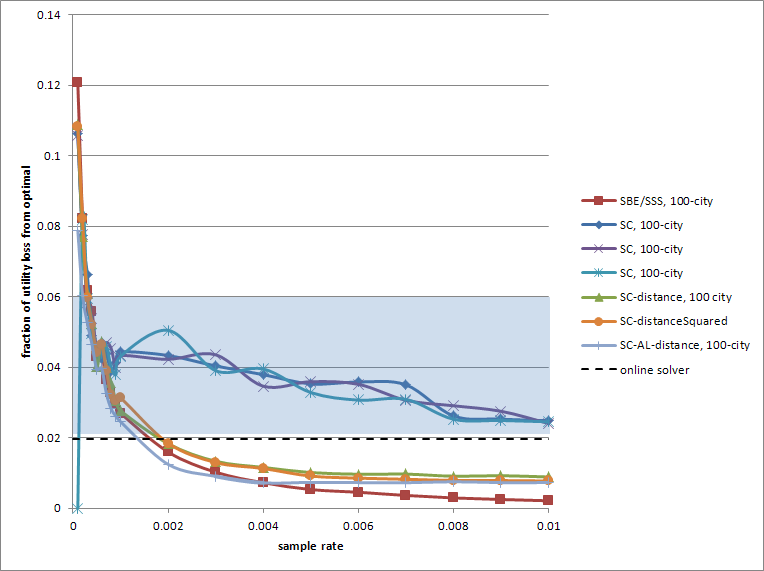
\includegraphics[scale=0.4]{pics/100tsp_baseline.eps}
\caption{Results of applying various approximation algorithms to the 100-city TSP domain.  The dotted line represents the utility loss of the online planner.  The shaded region is the expected loss of DTSP online repair algorithms as suggested by \cite{larsen2000dvrp}.}
\label{fig:100tsp_baseline}
\end{center}
\end{figure}

\subsection{SC+Bias} 

Based on the results of the SC experiments, it became apparent that the larger solution regions tended to be represented in the approximated PS Map, but smaller regions tended to disapppear.  This occurred due to the lower probability of the initial random sample choosing a problem instance in that region, resulting in either a particular region not being represented in discovered solutions or probable solutions being assigned.  One attempt to mitigate this effect was inspired by observing that within the high-quality PS Map, more rapid changes in solutions and smaller solution regions tend to exist near city locations.  The SC+bias algorithm attempts to take advantage of this observation by biasing samples towards the regions near cities.  The city radius and bias parameters determine, respectively, the radius of the region around a city to apply the bias and how much to bias the samples.  The near-city region is defined as a circle with the specified radius.  The bias represents the odds that the near-city region will be sampled.  For example, a bias value of three indicates that the near-city region will be sampled with odds 3:1 versus the non-near-city region.  

\subsubsection{Experiment Parameters} This experiment approximated a PS Map for a 100-city DTSP.  I assigned a bias factor as integers in the range from one to five, inclusive, and the city radius in the range from one to five, inclusive. The approximation algorithm was executed ten times for each combination of bias factor and city radius.

\subsubsection{Results} The results of this experiment are shown in Figures \ref{fig:scbias-results-all} and \ref{fig:scbias-results-100city-005sample}.  These results do not appear to show an obvious pattern to determine which parameters are most promising.  For example, the best performance are at the valleys (recall that lower utility loss is preferred)  at bias values of one, four, and five, and radius values of two, four, and five.  Looking at the graph, there is not an obvious gradient to suggest a generalized rule for setting these parameters.


\subsection{SC+AL} 


Sampling classification with active learning (SC+AL) is another attempt to allow for smaller solution regions to be approximated effectively.  SC+AL may be considered a generalization of SC+bias in that it allows more concentrated sampling in regions of the problem space in which the classification appears ambiguous rather than limiting the targetted samples to predetermined locations.  For example, if two solutions are both strong candidates to be assigned to a specific problem instance, then SC+AL would solve the problem instance rather than risk assigning an incorrect solution.  Similarly, if there are no strong candidates for a particular problem instance, then SC+AL would allow the problem instance to be solved rather than assign an arbitrary solution to it.  

\subsubsection{Experiment Parameters}  The alpha parameter was set to 0.5.  Thus, half of the allotted problem instances solved were selected with random sampling.  The other half were reserved for problen instances that the algorithm determines to be ambiguous.

\subsubsection{Results} The results of this experiment are shown in Figure \ref{fig:100tsp_baseline}.  At the lower sample rates, the performance of the SC+AL algorithm appears to be slightly better than the SC results.  This could suggest that at low sample rates, it is more critical to choose samples that convey the most information about the solution space.  It's reasonable that as the sample rate increases, the probability increases of obtaining that same sample information through chance.


\subsection{SSS} 

\subsubsection{Experiment Parameters}  No algorithm-specific parameters were required for this experiment.  As with the other experiments in this domain, the sample rate ranged from .0001 to .01 for a problem space consisting of 100-city DTSPs containing one variable city.

\subsubsection{Results} The results of this experiment are shown in Figure \ref{fig:100tsp_baseline}.  The utility loss of SSS quickly drops, and at sample rates greater than .003 becomes the best performing algorithm.  Intuitively, this seems reasonable:  assuming that the initial sample discovers most solutions, then testing each of the solutions against the problem instance would result in the problem instance being assigned the optimal solution.


\subsection{SBE} 

The solution border estimation algorithm (SBE) considers the mathematical features of the TSP.  It calculates the border by recognizing that the border between any two solutions is represented by equating the distance functions of the two solutions.  Unfortunately, at the time of this experiment, I did not find a Java library that could solve the complex equations that resulted from this technique.  The SBE-trace technique is inspired by SBE; however, it finds borders between two solutions by searching the space between two problem instances with known solutions.  Thus, a binary search can be employed.  Assuming that the border between two solutions is continuous, then the remainder of the border can be found by comparing the utility of the two solutions at each problem instance. 

\subsubsection{Experiment Parameters}  

No algorithm-specific parameters were required for this experiment.  As with the other experiments, the sample rate ranged from .0001 to .01 for a problem space consisting of 100-city DTSPs, with one city having variable location.

\subsubsection{Results}  The results of SBE-trace are shown in Figure \ref{fig:100tsp_baseline}.  Note that SBE-trace is only suitable for two-dimensional PS Map approximation.  Because of this limitation, it is not applicable to most domains, and thus I did not emphasize this algorithm in the subsequent experiments, which have PS Maps with higher dimenstions.


\subsection{SVM} 

The support vector machine algorithm (SVM) uses a support vector machine to try to generalize the idea of SBE to multiple dimensions.  Support vector machines calculate a maximum margin plane to separate different classes.  The observations in this application are the sampled problem instances labeled with their solutions.  

\subsubsection{Experiment Parameters}

No algorithm-specific parameters were required for this experiment.  As with the other experiments, the sample rate ranged from .0001 to .01 for a problem space consisting of 100-city DTSPs, with one city having variable location.

\subsubsection{Results}  The results of this approach are in figure X.

\subsection{SVM+SBE} 

One disadvantage of the SVM-based approach is that it can misclassify problem instances.  SVM determines the borders between two solution regions by creating a margin as far as possible between known solution instances.  This process results in a border that is approximately midway between known solutions.  SVM has been shown to be a good optimization technique in general; however, it does lead to misclassifications when the actual border does not conform to this approximation.  By applying additional samples in key locations, the bounds of the margins calculated by the SVM can be made tighter and thus more consistent with the acutal borders.  In this approach, the first step is an initial set of problem instances that are sampled and solved. The second step applies the binary search used in the SBE-trace algorithm to each distinct pair of solutions, resulting in problem instances that represent solutions on the border between the distinct pair of solutions.  Finally, those problem instances and the labeled solutions are added to the training set for the SVM. 

\subsubsection{Experiment Parameters} 

The alpha parameter, which determines the fraction of the total allocated sample that will be used during random initial sampling, was set to 0.5.

\subsubsection{Results} The results of this approach are in figure X. 




\begin{figure}
\begin{center}
\includegraphics[scale=1.0]{pics/scbias-results-all.eps}
\caption{Average utility loss of approximate PS Maps generated by SC+bias for DTSP problems of various sizes.}
\label{fig:scbias-results-all}
\end{center}
\end{figure}

\begin{figure}
\begin{center}
\includegraphics[scale=1.0]{pics/scbias-results-100city-005sample.eps}
\caption{Average utility loss of approximate PS Maps generated by SC+bias for 100-city DTSP problems at sample rate .005.  SC-generated PS Maps generated under identical conditions have an average accuracy of .035.}
\label{fig:scbias-results-100city-005sample}
\end{center}
\end{figure}


\subsection{Analysis}

These results show that these algorithms are comparable to or better than online repair performance:  all of the algorithms except for SC perform better than online repair at sample rates of .002 and above.  It is quite reasonable that the alternate algorithms would perform better than SC, because SBE and SC+AL proactively attempt to find key problem instances that distinguish one solution from another, and SSS considers more information than SC during classification.  The fact that the distance-squared version of SC performs better than the others suggests that solved problem instances that are closer to the instance being classified are more indicative of the proper solution than solved problem instances that are further away.

The results for SC+bias applied to TSP of various sizes are shown in Figure \ref{fig:scbias-results-all}.  Again, the results are comparable to online repair, but not as good as other techniques.  SC+bias has \textit{bias factor} and \textit{city radius} parameters that can be modified and were set to various values within the experiment.  Bias factor represents the degree to which to bias sampling to be near a city.  The city radius indicates how close a problem instance has to be to a city to potentially benefit from the bias.  Figure \ref{fig:scbias-results-100city-005sample} shows utility loss results at sample rate .005 when SC+bias is applied with a range of parameter configurations.  The results vary widely, and there does not appear to be any obvious correlation between specific parameter settings and the utility loss.  This behavior also appears reasonable.  The goal of this algorithm was to attempt to exploit city locations as indicators of boundaries between solution regions.  However, there are many solution regions that are not near cities; thus, this algorithm has uneven and limited benefit.

The early experiments demonstrate that SSS and SBE have the best performance.  SBE's performance is perhaps expected, as this algorithm most directly finds solution regions, thus exploiting the characteristic of this domain space in which similar problem instances tend to have similar solutions.  Alternatively, SSS's performance is best attributed to its brute-force approach of examining every problem instance and testing all known solutions.  This would seem to continue to be feasible with a tractable number of problem instances and solutions, but may not scale well.  Figure \ref{fig:sss-results-all} explores SSS and SBE's potential with additional problem sizes.  The performance continues to be good for all problem sizes, but appears to converge more rapidly for the smaller problem sizes.  This behavior is expected due to the small number of unique solutions and larger homogeneous regions.



% Not sure why these two paragraphs are here

%Results for the approximation algorithms SC, SC+AL, SSS, and SBE when applied to 100-city TSP high-quality maps are displayed in Figure \ref{fig:100tsp_baseline}.  The algorithms with ``-distance'' and ``-distanceSquared'' represent variants in which the weighting of the neighbors in the  nearest-neighbor polling is decreased as a function of the distance or distance squared from the problem take more information into account during classification.  The fact that the distance-biased versions of SC also perform better means that problem instances that are closer to the problem instance being classified are far more likely to have a similar solution than more distant problem instances.




\begin{figure}
\begin{center}
\includegraphics[scale=1.0]{pics/sss-results-all.eps}
\caption{Average utility loss of approximate PS Maps generated by SBE and SSS for DTSP problems of various sizes.}
\label{fig:sss-results-all}
\end{center}
\end{figure}



%Focusing on the 100-city TSP as most representative of a complex domain, Figure \ref{fig:tsp-svmsbe-100city} shows the performance of SVM+SBE against a 100-city TSP high-quality PS Map for two different alpha values.  The performance is not as good as the SBE and SSS algorithms.

% source C:\Documents and Settings\holderh1\My Documents\umbc\journalPaper\pics

%\begin{figure}
%\begin{center}
%\includegraphics[scale=1.0]{pics/tsp-svmsbe-fractional-loss-vs-sample-rate.eps}
%\caption{Average utility loss of approximate PS Maps generated by SVM+SBE for 100-city DTSP problem.}
%\label{fig:tsp-svmsbe-100city}
%\end{center}
%\end{figure}




\section{Knapsack Problem}

The knapsack problem is a combinatorial optimization problem in which a subset of items of variable weight and value are chosen such that the total value is maximized and the total weight falls below  a given threshold.  For this experiment, I use the 0-1 knapsack problem variant, in which either zero or one copies of each item may be placed in the knapsack.  The knapsack is prepopulated with a set of items that utilize 396 dekagrams (dag) of the total knapsack capacity of 400 dag, and one or more items  of varying value and weight is added to the pool of items.

The knapsack domain demonstrates the applicability of the algorithms in a different domain.  One difference between this domain and the TSP domain is that it entails a more abstract representation of distance, as an item's  weight and value characteristics do not directly correspond to location and  distance as do the cities within the TSP domain. The high-quality solution PS Map's characteristics also differ in this domain.  For example, looking at the high-quality PS Map, one can see that, whereas the TSP domain had very circular homogeneous regions, the knapsack domain has rectangular homogeneous regions.  I apply the same algorithms to this domain, with the exception of the SBE-trace algorithm, which is only suitable for problem spaces of two dimensions.  I expect that performance of the algorithms could be worse in this domain, due to the greater number of solutions and smaller solution region size.



\subsection{High-Quality PS Map} For the  experiment, I defined a set of 22 items, each with known weight and value characteristics as shown in Table \ref{tab:knapsack-item-pool}, from which to maximize the value of the knapsack while conforming to its maximum weight capacity.  I defined one additional item, varying the weight and value from 1-100 inclusive to create 10,000 ($\textrm{100}^{\textrm{2}}$) problem instances.  As a baseline, I solved all 10,000 problem instances to generate a high-quality PS Map.  As with the TSP domain, I applied SSS over the PS Map to reduce errors from the heuristic solver.  A visualization of the resulting two-dimensional PS Map is depicted in Figure \ref{fig:knapsack-ideal}.

I then generated more complex problem spaces  by adding multiple items of varying weight and value characteristics to the pool.  Solving each of the resulting problem instances -- consisting of the static items and two additional items -- resulted in a four-dimensional PS Map consisting of two weight and two value dimensions.  I generated a high-quality PS Map, solving all 176,400 ($20^2 \times 21^2$) problem instances.  

Continuing, I generated an eight-dimensional problem space consisting of a weight and value axis for each of four variable items.  The range of the weight was 16 to 20 inclusive and the range of the value was 31 to 35 inclusive, resulting in a problem space of $5^8 = 390,325$ problem instances.  For each of the problem instances in the problem space, I created the full problem instance by adding the variable items indicated by the problem instance to the knapsack.  For example, if a problem instance in the problem space is $(w_0,v_0,w_1,v_1,w_2,v_2,w_3,v_3)$, then I solved a knapsack problem consisting of the pool of items in Table \ref{tab:knapsack-item-pool} plus items with weight and value scores of $(w_0,v_0),(w_1,v_1),(w_2,v_2),$ and $(w_3,v_3)$.  I solved each of the knapsack problems and created a mapping from each of the instances in the problem space to each of the calculated solution, thus composing the PS Map.

Finally, I generated a second PS Map of an eight-dimensional problem space as above, but with the range of the weight expanded by one unit to 15 to 20, resulting in a problem space of $6^4 \times 5^4 = 810,000$ instances.

\begin{figure}
\begin{center}
\includegraphics[scale=.2]{pics/knapsack-400-ideal-with-labels.eps}
\caption{High-quality PS Map for a knapsack problem.  Best viewed in color.}
\label{fig:knapsack-ideal}
\end{center}
\end{figure}

\subsection{Online Repair Baseline}  The online repair method is a greedy solver that selects the item with the highest value-to-weight ratio.


\subsection{Experiment Parameters}

The knapsack problem tested the sampling-classification (SC), sampling-classification with active learning (SC+AL), support vector machine (SVM), support vector machine with solution border estimation (SVM+SBE), and select from sampled solutions (SSS) methods.  I did not perform experiments with SBE because, as previously mentioned, it is only applicable for two-dimensional domains, and, thus, is not as useful in general cases.  The SC+Bias approximation algorithm is also omitted because its application is specific to the TSP domain's city location parameters, and there is not a clear analog within the knapsack domain.

In my experiments, I found that large regions of the problem space were homogeneous, particularly as the values of the problem instances' variable features increase.  To avoid positively skewing the results, I chose feature ranges to focus on the more heterogeneous regions of the problem instance space.  For the two-dimensional experiment, I limited the problem space to problem instances with  weights from  1-20, inclusive, and values from 50-70, inclusive.  For example, when considering only one additional item, the first problem instance would consist of the static items plus an additional item with a weight and value (1,50); the second problem would consist of the static items plus an additional item with weight and value (2,50); and so forth, accounting for all possible combinations.

The approximation of all maps was done for  sample rates ranging from .0001 to .001.  For the SC+AL and SVM+SBE algorithms, the alpha rate was set to 0.5.  Thus, the initial sample rate is half of the allocated samples, leaving half for active sampling.  As before, the evaluation of the approximation is the fraction of the utility lost with respect to the heuristically calculated heuristic solution.


\begin{table}
\begin{center}
  \begin{tabular}{|p{5cm}|p{1.5cm}|p{1.5cm}|}
    \hline
    \textbf{Object} & \textbf{Weight} & \textbf{Value} \\ \hline
    apple & 39 & 40 \\ \hline
    banana & 27 & 60 \\ \hline
    beer & 52 & 10 \\ \hline
    camera & 32 & 30 \\ \hline
    cheese & 23 & 30 \\ \hline
    compass & 13 & 35 \\ \hline
    glucose & 15 & 60 \\ \hline
    map & 9 & 150 \\ \hline
    note-case & 22 & 80 \\ \hline
    sandwich & 50 & 160 \\ \hline
    socks & 4 & 50 \\ \hline
    sunglasses & 7 & 20 \\ \hline
    suntan cream & 11 & 70 \\ \hline
    t-shirt & 24 & 15 \\ \hline
    tin & 68 & 45 \\ \hline
    towel & 18 & 12 \\ \hline
    trousers & 48 & 10 \\ \hline
    umbrella & 73 & 40 \\ \hline
    water & 153 & 200 \\ \hline
    waterproof overclothes & 43 & 75 \\ \hline
    waterproof trousers & 42 & 70 \\
    \hline
  \end{tabular}
  \caption{Knapsack static item pool}
  \label{tab:knapsack-item-pool}
\end{center}
\end{table}

\subsection{Results \& Analysis}

The result of generating a high-quality PS Map is displayed in Figure \ref{fig:knapsack-ideal}.  The map confirms an intuitive estimation of solutions: for problem instances in which the variable item's weight falls within the slack of the  original solution, it is always included in the knapsack.  Once the variable item's weight exceeds the available slack, it is excluded from the knapsack until it becomes valuable enough to replace an item currently in the knapsack.  Moving along the weight dimension, the variable item remains in the knapsack until it becomes too heavy for its value to contribute to an optimal solution and is excluded from the knapsack.  This pattern repeats, creating a set of solutions resembling a staircase of solutions, the edges of which represent a boundary in the solution space between where the variable item is included and excluded.

Figure \ref{fig:knapsack-2d-range01-loss} shows the results of applying the various PS Map approximation algorithms to a knapsack problem with one variable item.  As one might expect, most of the algorithms trend towards zero utility loss as the sample rate increases.  The notable exceptions are the SC and SSS algorithms. The SSS algorithm appears to provide somewhat of a theoretical best performance, with the other algorithms gradually converging.  The SC algorithm appears to have a much slower convergence, as it still shows a loss of approximately 20\% of the optimal utility at a 0.1 sample rate.  Figure \ref{fig:knapsack-2d-range001-loss} highlights the turbulent region up to and including sample rate 0.01.  Here it becomes apparent that the SC algorithm performs comparably to the other algorithms at this low sample rate, with the AL algorithm initially lagging behind.  Figure \ref{fig:knapsack-2d-range0001-loss} zooms in an additional time to the lower tenth of the sample rate range, up to and including 0.001, showing even more pronounced performance differences.  The SC, SVM, and SVM+SBE algorithms are generally grouped together, and the AL and SSS algorithms show a utility loss at a fairly constant level at opposite ends of the performance range.

Figures \ref{fig:knapsack-2d-range01-rank}, \ref{fig:knapsack-2d-range001-rank}, and \ref{fig:knapsack-2d-range0001-rank} show the relative rankings of the algorithms for the each of the preceding three figures.  Although the quantitative difference in performance is lost in these graphs, it does notionally illustrate the preferred algorithm as the sample rate increases.  We again see that the AL algorithms initially performs poorly, but converges quickly to become comparable to the SVM and SVM+SBE algorithms.  Conversely, the SC algorithm performance degrades and quickly becomes the worst algorithm. 

These results suggest that at very low sample rates, it is advantageous to use SC rather than AL, perhaps because SC's broader coverage of the space of problem instances is more useful than AL's targeted sampling for small sample rates.  However, at higher sample rates, the higher number of samples available for AL's initial sample appears to provide broad enough converage for the targeted sampling  to outperform the SC algorithm.  It is interesting that there is not the same level of distinction between SVM and SVM+SBE, perhaps because SVM's classifications methods permit the information gained from a sample to be applied more broadly, through the use of the maximum margin plane.  SC and AL, on the other hand, limit the use of a sample's information to a very localized region.  The advantage of SVM+SBE over SVM is that the targeted samples help to provide a more precise hyperplane location.  However, in the knapsack domain, in which the utilities of the available solutions are similar,  the benefit of the more precise hyperplane location is not as significant.  Additionally, the number of samples available for targeted sampling may not provide enough information to create a more precise margin, particularly as the number of dimensions increases.



%source C:\Documents and Settings\holderh1\My Documents\umbc\dissertation\data\k\recreateOldResults\scOutput_2011_10_01-typicalSampleRate.xlsx
%\begin{figure}
%\begin{center}
%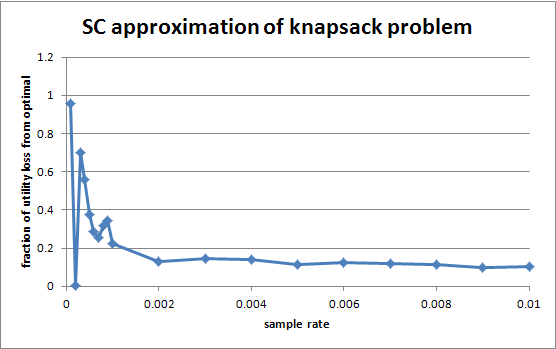
\includegraphics[scale=0.5]{pics/sc_knapsack.eps}
%\caption{SC applied to a two-dimensional knapsack problem domain.}
%\label{fig:sc_knapsack}
%\end{center}
%\end{figure}

%source C:\Documents and Settings\holderh1\My Documents\umbc\dissertation\data\recent\k_results-2d\Knapsack-2d.xlsx
%\begin{figure}
%\begin{center}
%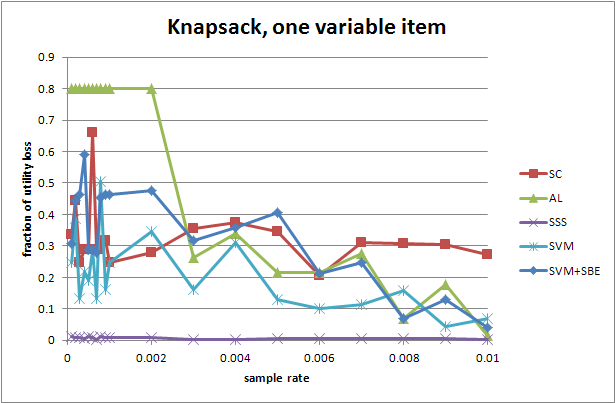
\includegraphics[scale=0.5]{pics/knapsack-2d.eps}
%\caption{Results of algorithms applied to a two-dimensional knapsack problem domain.}
%\label{fig:knapsack-2d}
%\end{center}
%\end{figure}

%C:\Documents and Settings\holderh1\My Documents\umbc\dissertation\data\recent\k_results-2d-n20-largeSampleSet/2d-n20-largeSampleSet.xlsx
\begin{figure}
\begin{center}
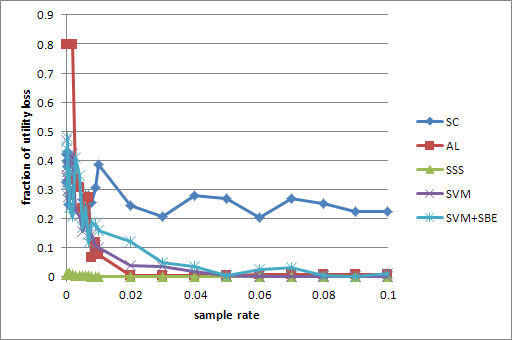
\includegraphics[scale=0.5]{pics/k-2d-n20-range01-loss.eps}
\caption{Results of algorithms applied to a two-dimensional knapsack problem domain.}
\label{fig:knapsack-2d-range01-loss}
\end{center}
\end{figure}

%C:\Documents and Settings\holderh1\My Documents\umbc\dissertation\data\recent\k_results-2d-n20-largeSampleSet/2d-n20-largeSampleSet.xlsx
\begin{figure}
\begin{center}
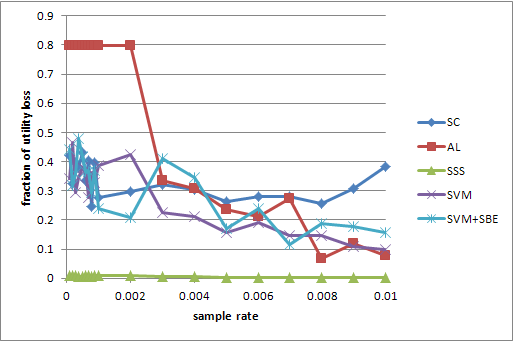
\includegraphics[scale=0.5]{pics/k-2d-n20-range001-loss.eps}
\caption{Results of algorithms applied to a two-dimensional knapsack problem domain, focus on sample rate .01 and lower.}
\label{fig:knapsack-2d-range001-loss}
\end{center}
\end{figure}

%C:\Documents and Settings\holderh1\My Documents\umbc\dissertation\data\recent\k_results-2d-n20-largeSampleSet/2d-n20-largeSampleSet.xlsx
\begin{figure}
\begin{center}
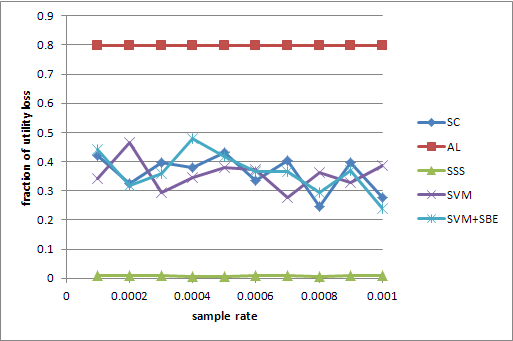
\includegraphics[scale=0.5]{pics/k-2d-n20-range0001-loss.eps}
\caption{Results of algorithms applied to a two-dimensional knapsack problem domain, focus on sample rate .001 and lower.}
\label{fig:knapsack-2d-range0001-loss}
\end{center}
\end{figure}

%C:\Documents and Settings\holderh1\My Documents\umbc\dissertation\data\recent\k_results-2d-n20-largeSampleSet/2d-n20-largeSampleSet.xlsx
\begin{figure}
\begin{center}
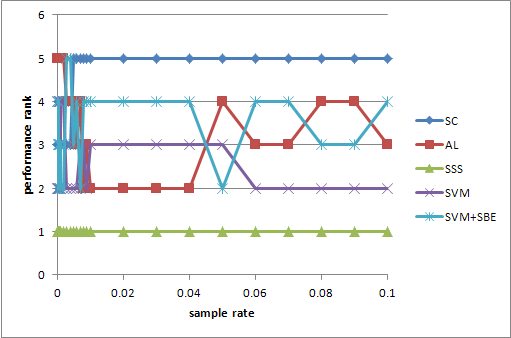
\includegraphics[scale=0.5]{pics/k-2d-n20-range01-rank.eps}
\caption{Ranking of algorithms applied to a two-dimensional knapsack problem domain.}
\label{fig:knapsack-2d-range01-rank}
\end{center}
\end{figure}


%C:\Documents and Settings\holderh1\My Documents\umbc\dissertation\data\recent\k_results-2d-n20-largeSampleSet/2d-n20-largeSampleSet.xlsx
\begin{figure}
\begin{center}
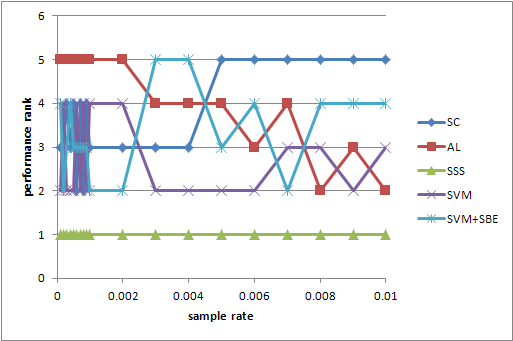
\includegraphics[scale=0.5]{pics/k-2d-n20-range001-rank.eps}
\caption{Ranking of algorithms applied to a two-dimensional knapsack problem domain, focus on sample rate .01 and lower.}
\label{fig:knapsack-2d-range001-rank}
\end{center}
\end{figure}

%C:\Documents and Settings\holderh1\My Documents\umbc\dissertation\data\recent\k_results-2d-n20-largeSampleSet/2d-n20-largeSampleSet.xlsx
\begin{figure}
\begin{center}
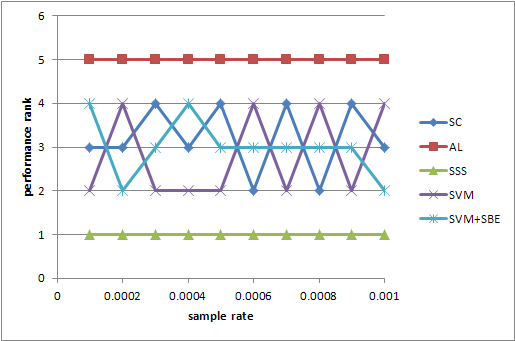
\includegraphics[scale=0.5]{pics/k-2d-n20-range0001-rank.eps}
\caption{Ranking of algorithms applied to a two-dimensional knapsack problem domain, focus on sample rate .001 and lower.}
\label{fig:knapsack-2d-range0001-rank}
\end{center}
\end{figure}

%\ref{fig:svmsbe_knapsack_4d_w14-24_v30-40}

Figure \ref{fig:knapsack-4d} shows the results of applying the PS Map approximation algorithms to a knapsack problem with two variable items.  Because each item has a weight and height characteristic, this results in a four-dimensional PS Map.  In this experiment, I limited the range of the weight and value of the items to [14,24] and [30,40], respectively, due to the computation time required to complete the experiment.  The graph shows a loss of utility well under 1\% at low sample rates.  In this domain, the algorithms appear to benefit from the higher dimensionality, because there is not a large increase in the number of unique solutions, leading to larger homogeneous solution regions that the algorithms can exploit.



The spikes in the SVM+SBE results are the effect of high variance that is a function of the manner in which SVM+SBE selects its sample points and the structure of the knapsack problem space.  After the initial random sampling, SVM+SBE uses its additional samples to find problem instances that correspond to borders between pairwise solutions. As a result, all of SVM+SBE's subsequent samples will be in a region of the problem space that is bounded by the initial sample set.  Therefore, if the initial sample does not bound a region that represents all solutions, then no subsequent samples will discover those solutions.  In this test case, the region had a total of four solutions.  If the initial sample discovered all four, then the average fraction utility loss was close to zero.  If the initial sample discovered only three solutions and none were feasible with respect to the unrepresented problem instances, then the average fraction utility loss rose to around 0.15.  If the initial sample discovered only two solutions, the average fraction utility rose to around .45, indicating that the library did not have a feasible solution for almost half of the problem instances.

This effect is less pronounced in the other algorithms.  For SC, SSS, and SVM, the probability of excluding a solution region at a particular sample rate is smaller because, unlike SVM+SBE, all of the samples are used in the initial sample, rather than a subset.  For AL, which, like SVM+SBE, also reserves a fraction of its samples for targeted sampling, its subsequent sampling targets unrepresented regions, thereby reducing the probability that a region of the problem space would remain unsampled.  The last factor is the domain, for which not all solutions are feasible for a given problem instance.  In contrast to TSP, in which any solution can be applied to any problem instance, the knapsack problem domain defines a hard constraint -- total weight -- that if  violated by a solution renders it inapplicable to the problem instance.  This characteristic leads to large losses of utility because an infeasible solution has a utility close to zero,\footnote{To avoid division-by-zero errors, the lowest utility in the knapsack problem domain is 1.} whereas in a domain like  TSP, a poor solution still does still contribute some portion of the optimal utility.


Figure \ref{fig:knapsack-4d-zoom} highlights the area of the graph where several of the algorithms appear to have similar performance.  Upon closer inspection, the typical  rapid convergence of the SSS algorithm is again visible.  In this case, the other algorithms tend asymptotically towards zero utility loss as well.


%\begin{figure}
%\begin{center}
%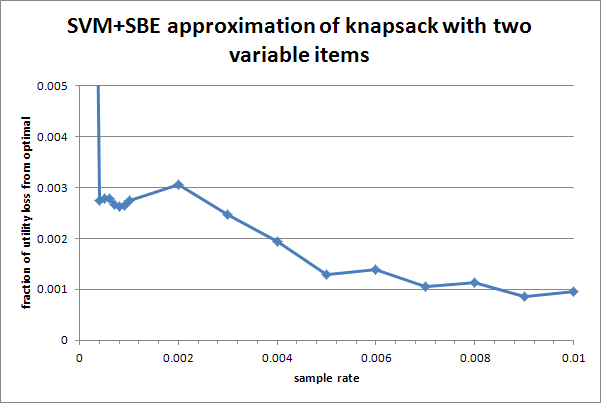
\includegraphics[scale=0.5]{pics/svmsbe_knapsack_4d_w14-24_v30-40.eps}
%\caption{SVM+SBE applied to a four-dimensional knapsack problem domain.  Problem space is limited to weight 14-24 inclusive and value 30-40 inclusive.}
%\label{fig:svmsbe_knapsack_4d_w14-24_v30-40}
%\end{center}
%\end{figure}

%C:\Documents and Settings\holderh1\My Documents\umbc\dissertation\data\recent\k_results-4d\Knapsack-4d.xlsx
\begin{figure}
\begin{center}
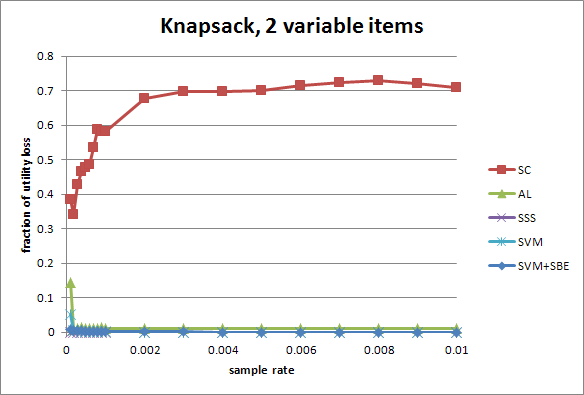
\includegraphics[scale=0.5]{pics/knapsack-4d.eps}
\caption{Results of algorithms applied to a four-dimensional knapsack problem domain.}
\label{fig:knapsack-4d}
\end{center}
\end{figure}

%C:\Documents and Settings\holderh1\My Documents\umbc\dissertation\data\recent\k_results-4d\Knapsack-4d.xlsx
\begin{figure}
\begin{center}
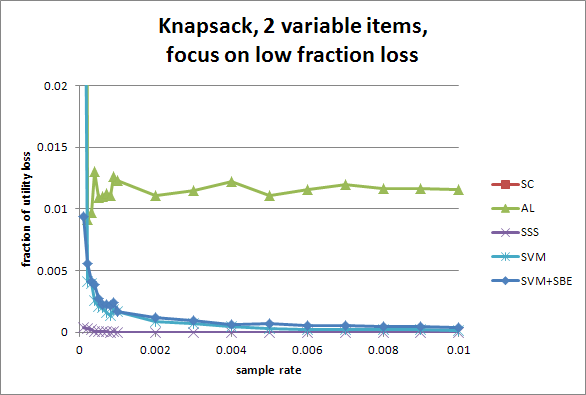
\includegraphics[scale=0.5]{pics/knapsack-4d-zoom.eps}
\caption{Results of algorithms applied to a four-dimensional knapsack problem domain, highlighting low utility loss.}
\label{fig:knapsack-4d-zoom}
\end{center}
\end{figure}


Figure \ref{fig:svmsbe_knapsack_4d_baseline} puts these results in context against various baselines.  The taller blue bars represent the fraction of utility lost if one were to assume a PS Map consisting of a single solution.  Because the high-quality PS Map had seven solutions, there are seven cases represented in the graph.  In this scheme, it is possible that the penalty for plan infeasibility could dominate the error results.  The shorter red bar represents the result of applying a default solution to a problem instance, but allows the system to choose an alternate solution if the default solution violates the weight threshold of the knapsack. In this case, a feasible plan is randomly chosen.  The upper dotted line represents the fraction of utility loss of SVM+SBE at a sample rate of .004.  The lower dotted line represents the identical loss of the online repair method as well as when sampling at a rate of .006 using SVM+SBE.  The online repair method is a greedy solver that selects the items with the highest value to weight ratios.  This demonstrates that the performance of the SVM+SBE algorithm when sampling at rate of .006 is roughly equivalent to that of the online repair technique.


%source: C:\Documents and Settings\holderh1\My Documents\umbc\dissertation\data\k\svm_4d\Results-baseline.xls
\begin{figure}
\begin{center}
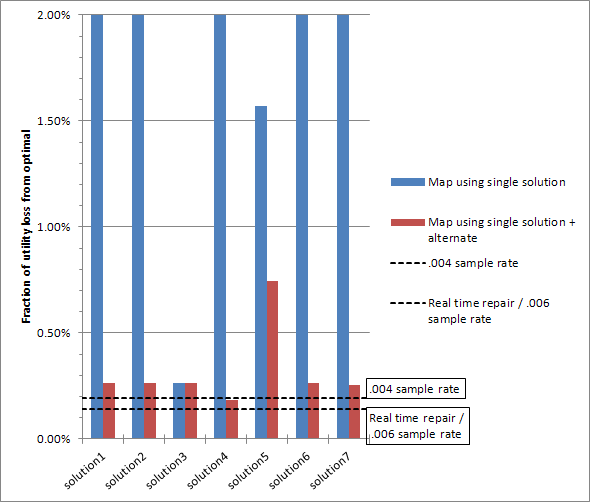
\includegraphics[scale=0.4]{pics/svmsbe_knapsack_4d_baseline.eps}
\caption{Results of applying SVM+SBE to a knapsack with two variable objects.  Dotted lines indicate fractional utility loss for online repair, .004 sample rate, and .006 sample rate, as labeled.  Bars indicate the fractional loss when using a default map consisting of either a single default solution, or a default solution and the best found feasible solution.}
\label{fig:svmsbe_knapsack_4d_baseline}
\end{center}
\end{figure}



%\begin{figure}
%\begin{center}
%\includegraphics[scale=.9]{pics/approach-results-100city.eps}
%\caption{Average utility loss of approximate PS Map generated by various approaches for 100-city DTSP problems}
%\label{fig:approach-results-100city}
%\end{center}
%\end{figure}




%\begin{figure}
%\begin{center}
%\includegraphics[scale=1.0]{pics/sss-results-all.eps}
%\caption{Average utility loss of approximate PS Maps generated by SBE and SSS for DTSP problems of various sizes}
%\label{fig:sss-results-all}
%\end{center}
%\end{figure}


\section{Elevator Problem}

The final domain, a elevator passenger transport problem,  represents a more traditional planning domain.  The TSP and knapsack domains can be considered optimization problems as well as planning problems.  The elevator domain  falls into the more traditional realm of planning, in which one has to find steps to accomplish a goal but  there is no direct mathematical representation of the domain.  Also, this domain is expected to be more challenging for the algorithms because the homogeneous regions are likely to be smaller and less regular.  Lastly, this domain represents  another level of abstraction, in that the solutions that are applied to the domain are not necessarily those that the algorithms will operate upon; the experiment parameters section describes this issue in detail.  I also apply the algorithms to this domain, again with the exception of SBE-trace.  I expect that this domain will the most challenging of the three, due to the possibility of changes in optimal plan being very sensitive to changes in the problem instance configuration.



The elevator domain is used by ICAPS in its International Planning Competition.  It specifies several elevators, floors, and passengers, and requires the planner to deliver the passengers from their starting floor to their destination floor at the lowest possible cost.  Each elevator is either ``fast'' or ``slow.''  The slow elevators incur little cost for movement, but more for stopping and starting.  Conversely, the fast elevators incur more cost for movement, but little for stopping and starting.  The planner specifies movements for the slow elevators, which may stop at any floor within a defined contiguous ``block'' of floors, and the fast elevators, which traverse the entire range of  floors, but only stop at block centers and boundaries.  For example, for a 12-floor problem with two slow elevators, one slow elevator will travel between the bottom six floors, and the other slow elevator will travel between the top six floors.  The fast elevator will travel throughout the floors, but only stop at floors 0, 3, 6, 9, and 12.  More formally, these features are specified with  M and N parameters, which create a problem domain with  M+1 total floors in blocks of N+1 floors, with fast elevators that may stop at floors that are multiples of $\frac{N}{2}$.  Thus, in the example above, M is 12 (13 floors from 0 to 12) and N is 6 (two blocks each of seven floors, one from 0 to 6 inclusive, the other from 6 to 12 inclusive).  

Typically, each planner submitted to the competition targets either the ``optimal'' or ``sacrificing'' track. The ``optimal'' track requires a planner to find the least costly means of transporting the passengers to their destinations.  The ``sacrificing'' track does not require a planner to find the optimal plan, but only to find a feasible plan to deliver all of the passengers.  My experiments focused on the optimal track and used one of the more successful planners, the LAMA Planner \citep{richter2010lama}.

\subsection{High-quality PS Map generation}  For this domain, I generated a 12-floor and two 24-floor elevator problems.  The 12-floor problem contained two seven-floor blocks (M=12, N=6), two slow elevators, and one fast elevator.  Each problem assumed two passengers with variable starting position, creating 169 problems to be solved with the LAMA planner.  One 24-floor configuation consisted of six five-floor blocks (M=24, N=4), and the other contained four seven-floor blocks (M=24, N=6).  The 24-floor problems vary the starting location of three passengers, thereby creating a high-quality map of 216 (i.e., $6^3$) problem instances.


Similar to other hard problems, planners in this domain employ heuristics in order to solve these intractable problems, and thereby benefit from ``smoothing'' as described in Section \ref{sec:sss}:  when generating the high-quality PS Map, each of the solutions is evaluated against each of the problem instances, and, if necessary, the problem instance is assigned a new solution.  This prevents the odd phenomenon of the occasional approximate solution having better utility than the ``optimal'' solution, which may skew the results.

\subsection{Experiment Parameters} My initial experiment used the 12-floor problem with three passengers, two slow elevators, and one fast elevator.  I varied the starting positions of two passengers, resulting in a 169-instance problem space.  In my initial experiment, there were too many unique plans, and the algorithms could not create classifications from the sampling. To make this domain appropriate for the algorithm, I abstracted the plans to transform a plan that moves elevators to a specific floor into a plan to move elevators to the location of specific passengers, thus creating a plan that could be applied to other problem instances.  For example, consider a raw plan with the steps

\begin{verbatim}
(move-down-slow slow0-0 n6 n0)
(board p0 slow0-0 n0 n0 n1)
(move-up-slow slow0-0 n0 n3)
(leave p0 slow0-0 n3 n1 n0)
\end{verbatim}

\noindent
This plan specifies that, first, the slow elevator with id slow0-0 moves from floor 6 to floor 0.  Next, the passenger with id p0 boards the elevator at floor 0, and the number of passengers increases from 0 to 1.  Then the elevator moves from floor 0 to floor 3, and in the final step, the passenger leaves the elevator at floor 3 and the number of passengers in the elevator decreases from 0 to 1.

In order to make this plan reusable, it is transformed to be  more general:

\begin{verbatim}
elevator slow0-0 picks up passenger p0
elevator slow0-0 drops off passenger p0
\end{verbatim}

The first step specifies that the elevator with id slow0-0 moves to passenger p0's current location, and p0 boards the elevator.  The second step then specifies that the elevator moves to passenger's desired destination and the passenger disembarks.  This general plan can  be applied to problem instances in which the elevator and passengers are on floors other than those assumed by the raw plan.

In addition to abstracting the plans, I normalize the plan so that differences in the ordering of independent actions are not interpreted as distinct plans.  For example, consider the plan below, annotated with action ids for ease of reference: 

\begin{verbatim}
1: elevator slow0-0 picks up passenger p0
2: elevator slow1-0 picks up passenger p1
3: elevator slow0-0 drops off passenger p0
4: elevator slow1-0 drops off passenger p1
\end{verbatim}

Note that the only dependencies are that action 1 must occur before action 3, and action 2 must occur before action 4.  Thus, there are six potential plans\footnote{(1,2,3,4), (1,2,4,3), (1,3,2,4), (2,1,3,4), (2,1,4,3), and (2,4,1,3)} representing the same overall process.  I normalize the plan by grouping together as many actions as possible that are performed by the same elevator.  In this case, the resulting normalization is:

\begin{verbatim}
1: elevator slow0-0 picks up passenger p0
3: elevator slow0-0 drops off passenger p0
2: elevator slow1-0 picks up passenger p1
4: elevator slow1-0 drops off passenger p1
\end{verbatim}

My subsequent experiments used a 24-floor elevator problem with six passengers, three of which had variable starting locations.  One experiment used six fast elevators and three slow elevators, and the other used four slow elevators.

\subsection{Online Repair Baseline} As a baseline, I implemented an online repair algorithm.  \cite{krogt05planrepair} describe plan repair as consisting of removing actions from the original plan that conflict with or impede achieving the new goal, followed by adding actions to the original plan that allow it to achieve the new goal.  My baseline online replanning algorithm is consistent with this methodology.  The new goal changes the initial location of the passenger, and thus I consider all actions that reference that passenger as candidates for deletion.  \citeauthor{krogt05planrepair} suggest that heuristics should be used to determine if a candidate action should be deleted.  My  heuristic is a simple one: I only remove the candidate action if it refers to a passenger whose starting position has moved outside the range of the elevator used by  the action.  For example, consider an abstracted action \textit{elevator slow0-0 picks up passenger p0}. Elevator slow0-0's range is floors n0 through n6. If this action is applied to a problem instance in which p0's starting position is n7 or above, then the action would be removed.

% TODO need a concrete example to clarify
In the event that an action is removed, I proceed with the second component of plan repair, in which I add actions to the original plan to achieve the new goal.  There are two alternatives for continuation:  either remove all subsequent actions that refer to the passenger and replan the entire route, or preserve the subsequent actions and replan the passenger route to comply with the constraints implied by the subsequent actions.  In the case of the former, I generate a solution to transport the passengers whose actions were removed.  In order to plan without the influence of the passengers whose actions have already been established, the initial starting conditions of those passengers is set to be equal to their destination location.  In the case of the latter, the final condition is set to the location expected by the action that moves the passenger to its final destination.  For example, if an action moves p2 from n6 to n2 to complete its journey, then the planner will set the final destination to n6.


\begin{algorithm}
%\caption{unrefinement strategy $<\mathcal{P},\mathcal{H}'> = \mathcal{D}(P,\mathcal{H})$\\Input: plan P and history $\mathcal{H}$\\Output: plan set $\mathcal{P}$ and updated history $\mathcal{H}'$}
\caption{Unrefinement}
\label{alg:p}

%\small
\begin{algorithmic}[1] 
  
  \For{each passenger p in plan P}
    \If{first action referencing p is invalid}
      \State remove all actions referencing p
    \EndIf
  \EndFor

\end{algorithmic}
\end{algorithm}


\begin{algorithm}
%\caption{refinement strategy $<\mathcal{P},\mathcal{H}'> = \mathcal{R}(P,\mathcal{H})$\\Input: plan P and history $\mathcal{H}$\\Output: plan set $\mathcal{P}$ and updated history $\mathcal{H}'$}
\caption{Refinement}
\label{alg:r}

%\small
\begin{algorithmic}[1] 
  \State {actions} $\leftarrow$ generate plan for deleted passenger actions
  \State parse and abstract {actions}
  \State add {actions} to P
  \State normalize P
\end{algorithmic}
\end{algorithm}


% I found that even with these plans, there were still too many distinct plans to allow SVM+SBE processing to be effective. I moved to a 24-floor problem instance in the hope that there would be larger regions of homogeneous plans that the SVM+SBE algorithm would be able to take advantage of.

%The 24-floor plan did not fit the constraints of the typical elevator domain problem, but this did not affect the planners.  It may have been an issue if were automatically generating the problem definition files, but I modified those by hand.

\subsection{Results}

Results from the 12-floor elevator problem domain are displayed in Figure \ref{fig:svmsbe_elevator_12}.  The dotted lines represent the fractional utility loss of three independent runs of the online repair algorithm described in Algorithms \ref{alg:p} and \ref{alg:r}.  The solid lines represent the results of applying the SVM+SBE approximation algorithm with various SVM kernels and the SSS algorithm.  The results demonstrate that the SSS algorithm has less fractional utility loss than the online algorithms, but the various SVM+SBE algorithms generally perform worse than the online repair algorithms.


Figures \ref{fig:elevator-3pass-maxsample05} through \ref{fig:elevator-3pass-maxsample001} show results of all the algorithms applied to the same 12-floor configuration mentioned above.  Again, the utility loss is much greater in this domain than in other domains.  This is due to the small number of unique solutions and the smaller size of homogeneous regions in the space.  This effect can be observed more explicitly by examining the performance of the algorithms in two different 24-floor configurations.  


%source:  C:\Documents and Settings\holderh1\My Documents\umbc\dissertation\lamaPlanner\work\p01-3d\results\svmElevatorOutput3D_2013_11_05__19_06_27-p01_3d-normalization.xlsx
%\begin{landscape}
\begin{figure}
\begin{center}
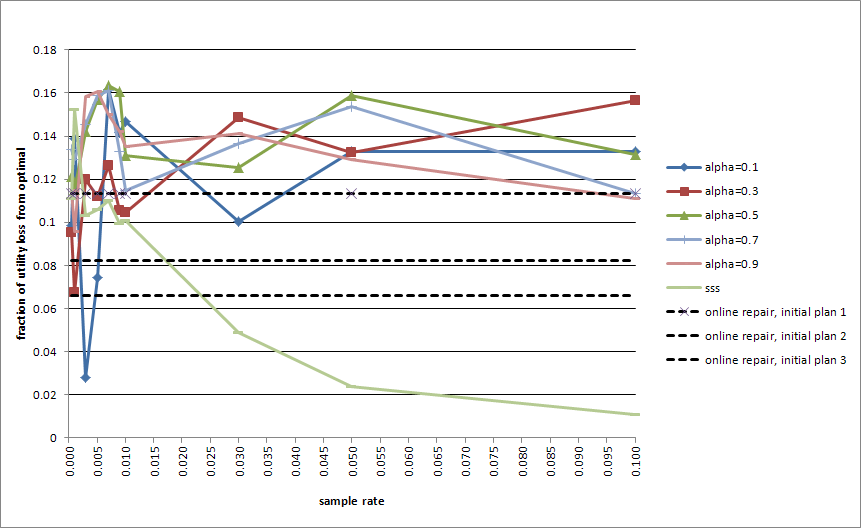
\includegraphics[scale=.5]{pics/svmsbe_elevator_12.eps}
\caption{Results of applying the SVM+SBE algorithm to a 12-floor elevator problem consisting of 2 slow elevators, 1 fast elevator, and 3 variable passenger starting locations.  Dotted lines represent the utility loss of online repair.  Solid lines represent approximations using various alpha values.}
\label{fig:svmsbe_elevator_12}
\end{center}
\end{figure}
%\end{landscape}




%source:     dissertation/lamaPlanner/work/p01-3d/results/nov8
\begin{figure}
\begin{center}
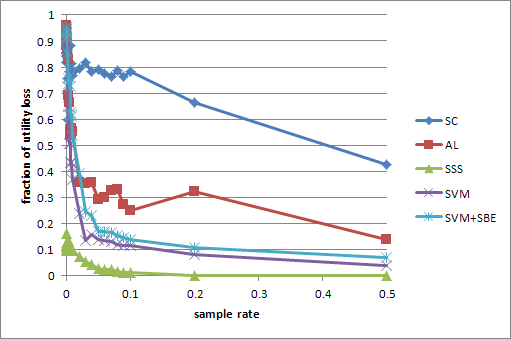
\includegraphics[scale=.5]{pics/elevator-3pass-maxsample05.eps}
\caption{Results of applying various approximation algorithms to a 12-floor elevator problem consisting of 2 slow elevators, 1 fast elevator, and 3 variable passenger starting locations.}
\label{fig:elevator-3pass-maxsample05}
\end{center}
\end{figure}

\begin{figure}
\begin{center}
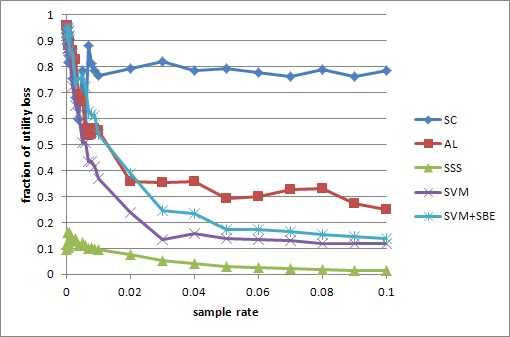
\includegraphics[scale=.5]{pics/elevator-3pass-maxsample01.eps}
\caption{Results of applying various approximation algorithms to a 12-floor elevator problem consisting of 2 slow elevators, 1 fast elevator, and 3 variable passenger starting locations, focus on sample rate 0.1 and lower.}
\label{fig:elevator-3pass-maxsample01}
\end{center}
\end{figure}

\begin{figure}
\begin{center}
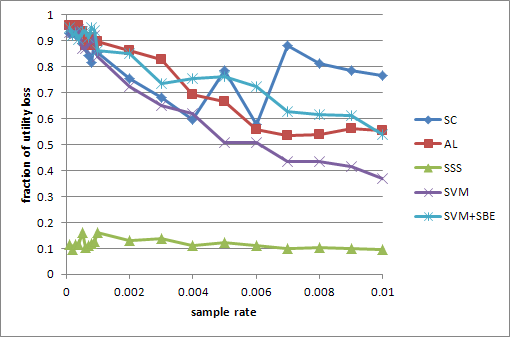
\includegraphics[scale=.5]{pics/elevator-3pass-maxsample001.eps}
\caption{Results of applying various approximation algorithms to a 12-floor elevator problem consisting of 2 slow elevators, 1 fast elevator, and 3 variable passenger starting locations, focus on sample rate 0.01 and lower.}
\label{fig:elevator-3pass-maxsample001}
\end{center}
\end{figure}





Results from the 24-floor elevator domain experiments are shown in Figures \ref{fig:elevator-6pass-maxsample05} through \ref{fig:elevator-6pass-nofast-maxsample001}.  These results show that for each problem configuration, SSS performs better than SVM+SBE.  Additionally, the algorithms perform better against the problem configuration with fewer elevators.  This is not unexpected,  given the nature of the problem space of each configuration and the algorithms used.  In all of the configurations, the problem spaces have homogeneous regions, but they are small, which can make it difficult for an SVM-based algorithm to converge and find the appropriate boundaries.  However, those small regions are not a disadvantage for the SSS algorithm, because it chooses a solution for each unsolved problem instance, rather than attempting to find groupings like SVM+SBE.  This same logic is applicable to the generally better results for the problem configuration with fewer elevators.  In the  configuration with four slow elevators, the homogeneous regions are larger than in the  problem space with six slow elevators, and thus the SVM+SBE algorithm performs better.  Because there are fewer total solutions in the configuration with fewer elevators, the SSS algorithm performs better as well.





\begin{figure}
\begin{center}
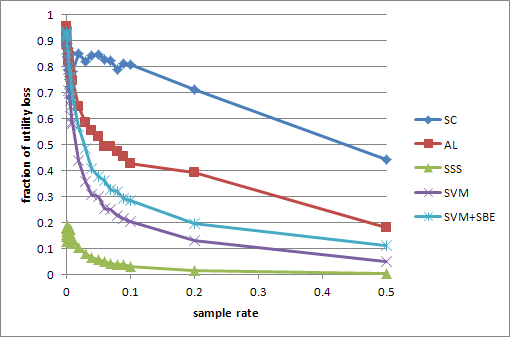
\includegraphics[scale=.6]{pics/elevator-6pass-maxsample05.eps}
\caption{Results of applying various approximation algorithms to a 24-floor elevator problem consisting of 6 slow elevators, 3 fast elevators, and 3 variable passenger starting locations of 6 total.}
\label{fig:elevator-6pass-maxsample05}
\end{center}
\end{figure}

\begin{figure}
\begin{center}
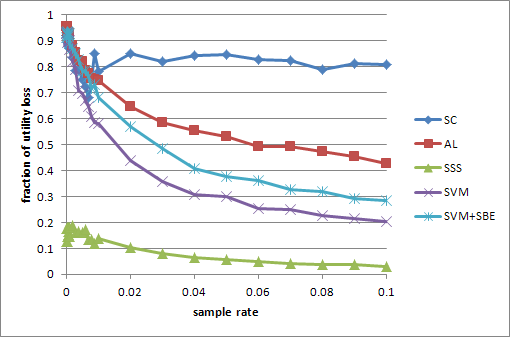
\includegraphics[scale=.6]{pics/elevator-6pass-maxsample01.eps}
\caption{Results of applying various approximation algorithms to a 24-floor elevator problem consisting of 6 slow elevators, 3 fast elevators, and 3 variable passenger starting locations of 6 total, focus on sample rate 0.1 and lower.}
\label{fig:elevator-6pass-maxsample01}
\end{center}
\end{figure}

\begin{figure}
\begin{center}
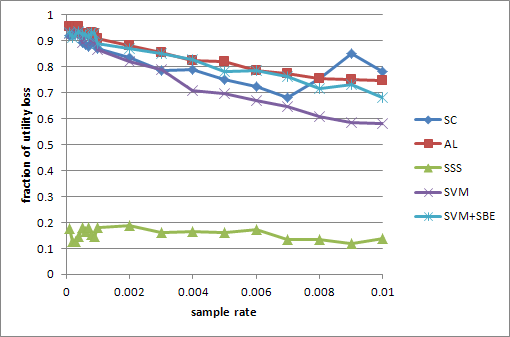
\includegraphics[scale=.6]{pics/elevator-6pass-maxsample001.eps}
\caption{Results of applying various approximation algorithms to a 24-floor elevator problem consisting of 6 slow elevators, 3 fast elevators, and 3 variable passenger starting locations of 6 total, focus on sample rate 0.01 and lower.}
\label{fig:elevator-6pass-maxsample001}
\end{center}
\end{figure}






%sources:  dissertation/lamaPlanner/work/p-6pass/results/nov8
%          dissertation/lamaPlanner/work/p-6pass-nofast/results/nov8
%          dissertation/lamaPlanner/work/p01-3d/results/nov8
\begin{figure}
\begin{center}
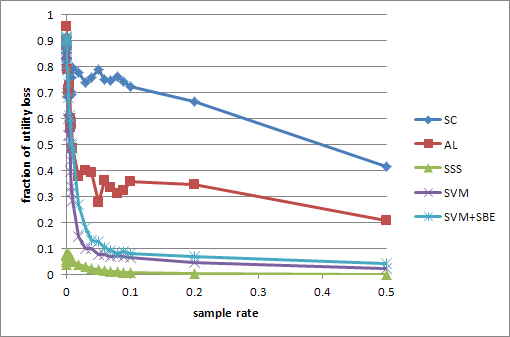
\includegraphics[scale=.6]{pics/elevator-6pass-nofast-maxsample05.eps}
\caption{Results of applying various approximation algorithms to a 24-floor elevator problem consisting of 4 slow elevators, 0 fast elevators, and 3 variable passenger starting locations of 6 total.}
\label{fig:elevator-6pass-nofast-maxsample05}
\end{center}
\end{figure}


\begin{figure}
\begin{center}
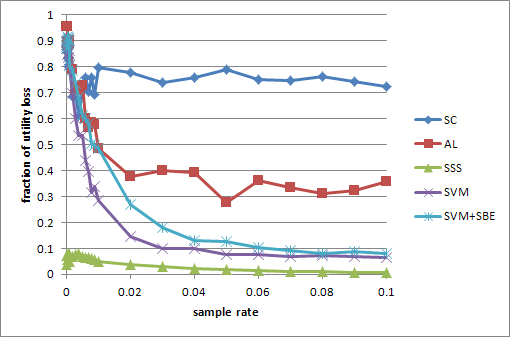
\includegraphics[scale=.6]{pics/elevator-6pass-nofast-maxsample01.eps}
\caption{Results of applying various approximation algorithms to a 24-floor elevator problem consisting of 4 slow elevators, 0 fast elevators, and 3 variable passenger starting locations of 6 total, focus on sample rate 0.1 and lower.}
\label{fig:elevator-6pass-nofast-maxsample01}
\end{center}
\end{figure}

\begin{figure}
\begin{center}
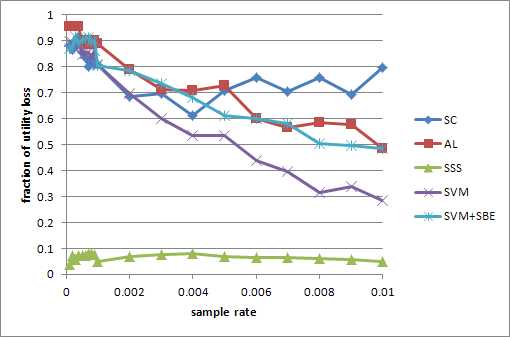
\includegraphics[scale=.6]{pics/elevator-6pass-nofast-maxsample001.eps}
\caption{Results of applying various approximation algorithms to a 24-floor elevator problem consisting of 4 slow elevators, 0 fast elevators, and 3 variable passenger starting locations of 6 total, focus on sample rate 0.01 and lower.}
\label{fig:elevator-6pass-nofast-maxsample001}
\end{center}
\end{figure}

%\begin{figure}
%\begin{center}
%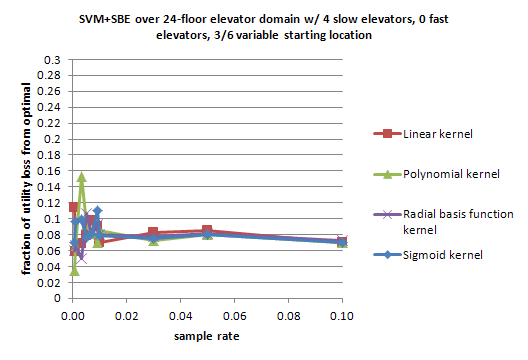
\includegraphics[scale=.6]{pics/svmsbe_elevator_4slow_0fast_6pass_3d.eps}
%\caption{Results of applying the SVM+SBE algorithm to a 24-floor elevator problem consisting of 4 slow elevators, 6 passengers, and 3 variable passenger starting locations.}
%\label{fig:svmsbe_elevator_4slow_0fast_6pass_3d}
%\end{center}
%\end{figure}



%\begin{figure}
%\begin{center}
%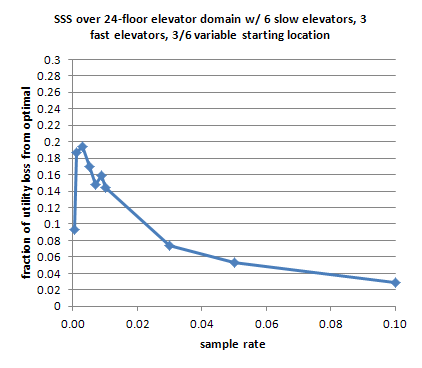
\includegraphics[scale=.6]{pics/sss_elevator_6slow_3fast_6pass_3d.eps}
%\caption{Results of applying the SSS algorithm to a 24-floor elevator problem consisting of 6 slow elevators, 3 fast elevators, 6 passengers, and 3 variable passenger starting locations.}
%\label{fig:sss_elevator_6slow_3fast_6pass_3d}
%\end{center}
%\end{figure}

%\begin{figure}
%\begin{center}
%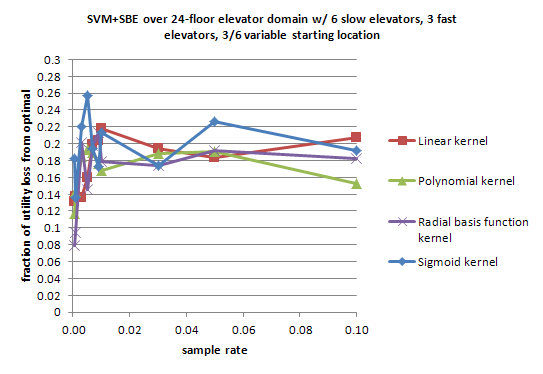
\includegraphics[scale=.6]{pics/svmsbe_elevator_6slow_3fast_6pass_3d.eps}
%\caption{Results of applying the SVM+SBE algorithm to a 24-floor elevator problem consisting of 6 slow elevators, 3 fast elevators, 6 passengers, and 3 variable passenger starting locations.}
%\label{fig:svmsbe_elevator_6slow_3fast_6pass_3d.eps}
%\end{center}
%\end{figure}


\section{Overall Analysis \& Discussion}

The results generally show little difference between approaches at low sample rates.  In fact, the results tend to be highly volatile, perhaps due to the high dependence on a small number of samples, which leads to large variances in the solutions available for the algorithms to consider.

SC tends to be a reasonable approach, with the added benefit that it is very simple to implement.  SC+bias shows the ability to improve on SC; however, it is not clear how to tune its parameters to achieve consistently good results.  SBE clearly is the best performer in the domains in which it was applied.  However, my implementation of SBE is limited to two dimensions.  SSS tends to have  the same results as SBE, but SSS is more computationally intensive, potentially leading to scaling issues in large problem spaces.  

The use of the SVM approach was intended to mimic the idea of SBE, but adds the ability to apply it higher-dimensional domains.  This approach tended to yield reasonable results.  Augmenting SVM with additional points to constrain the margin plane in SVM+SBE did not appear to have the significant impact one might have expected.  This may be because the test domains are fairly forgiving when applying a less optimal solution to a problem instance.  A domain in which there is a larger penalty for less optimal solutions may require an approach like SVM+SBE, which would provide a more accurate classification of solutions to the problem instances.  Although SVM and SVM+SBE did not achieve the results of SSS or SBE, they do have the advantage of being less computationally intensive and being applicable to domains of more than two dimensions.

The results of all algorithms appear to be sensitive to problem domain characteristics.  In the case of TSP, for example, larger size and a smaller quantity of homogeneous solutions regions generally resulted in better performance by the algorithms. This was also apparent when comparing the performance of the algorithms in the various elevator domain configurations.  The algorithms were able to perform well when tested against configurations that resulted in large homogeneous spaces in the solution space.

Most importantly, the results do demonstrate that these techniques are useful as an alternative to online plan repair.  At the appropriate sample rate, performance tends to be comparable, and sometimes better, than the online solution.  The benefit of my approach is that, assuming the ability to compute the necessary library before the environment changes, the new plan can be accessed much more rapidly than the online repairer can calculate a new plan.  These tradeoffs are discussed in more detail in the next chapter.


\chapter{Discussion}
\thispagestyle{plain}

\label{ch:application}

This chapter presents considerations when using the problem space analysis  (PSA) algorithms described Chapter \ref{ch:psa}.  It details some of the implicit criteria  for effective use of the algorithms, discusses the tradeoffs between using online repair and PSA, and describes other potential applications.

\section{Algorithmic Assumptions}
\label{sec:algorithmic-assumptions}


The effectiveness of the algorithms described in the previous chapters requires the existence of regions in the problem space with identical solutions.  Fewer regions and larger region size allow the algorithms to be more effective.  This was demonstrated through the experiments in which  TSPs with fewer cities created fewer, larger homogeneous solution regions and had better PS Map approximation.  Likewise, elevator domains with larger N values -- that is, larger blocks of floors -- tend to be more readily approximated by the algorithms.  Conversely, increasing the number of fast elevators potentially increases the number of regions, and, consistent with the results, becomes less amenable to approximation by the algorithms.

Additionally, the algorithms tend to assume some tolerance for error between neighboring solution regions.  Outside of solution border estimation, which attempts to mathematically define solution borders, all of the algorithms merely approximate the border between solutions.  A solution space in which there is a large utility difference between neighboring solutions is likely to negatively impact performance due to errors in determining the correct solution for problem instances near those solution border locations.  If the solution regions also are small, this would exacerbate the problem.

Thus, the algorithms rely on plan solution spaces containing homogeneous solution regions which the algorithms attempt to exploit.  These regions could be considered a function of a problem domain's objective function, as demonstrated by the justification for SBE.  Recall that the goal of SBE is to mathematically discover boundaries between solution regions by equating the objective functions of problem instances with differing variable features.  In this way SBE discovers problem instances for which two solutions have equal utility, thus constituting a boundary between two solution regions.  

As  seen with SBE and its skeletal generation of solution region boundaries, a TSP's solution boundaries are defined by each pairwise set of unique solutions discovered by an initial sample.  Fewer unique solutions increases the number of problem instances per solution; that is, it increases the size of the solution regions.  At a given sample rate, the larger solution regions create a greater likelihood that  a random sample will include the points necessary to identify the unique solutions within the problem space.

Other problem domains, such as the elevator domain, do not have explicit objective functions, but do have problem configurations that can serve the same purpose.  Within the TSP domain, the number of fixed cities affects the number of possible unique solutions, a fraction of which are represented in the problem space as solution regions.  In the knapsack domain, the set of static items affects the number of possible unique solutions as well.  As the value of a variable item increases, it eventually supersedes a  static item, resulting in a new solution.  For example, every problem instance in which the variable item is ``worse'' than the ``worst'' static item will have a solution that includes the static item rather than the variable item.\footnote{The evaluation of ``worse'' and ``worst'' depends on the heuristic used by the solver, but one example is the ratio of weight to value.}  The problem instances for which the variable item is ``better'' than the static item will result in a distinct solution.  Each static item presents an opportunity for a new solution. Thus, increasing the number of static items that are present in the domain results in  more distinct solutions and thereby more solution regions will exist.  

In the elevator domain, the number of blocks of floors affects the number of solution regions.  In general, the number of steps for a passenger to move from its starting to final destination is a function of the floor block that contains its starting location.  If abstracted as previously described, there is potentially little difference in the solution regardless of where in the floor block the passenger starts, which itself suggests an identical solution for several starting locations.  The greater number of floor blocks thereby leads to a greater number of solution regions.

The general conclusion is that the static characteristics have a direct impact on the number of homogeneous solution regions.  This can be observed in the previous examples in which the static characteristics tend to serve as an indicator of a threshold that variable features may cross and create a distinct solution.

In order to create these homogeneous regions, the axes used in the PS Map must be chosen appropriately, such that the problem instances with similar solutions are grouped together.  In the TSP domain, indexing by the x- and y-coordinates of the variable location resulted in homogeneous regions; in the knapsack domain, indexing by the variable item's weight and value results in homogeneous regions; and in the elevator domain, indexing by the starting passengers' starting location resulted in homogeneous solution regions.  In other domains, the surface attributes may not provide a natural grouping. For example, I briefly investigated the problem space of a game, \textit{Alien Frontiers}.    This game falls in the category of worker placement, in which a player rolls at least three and sometimes up to seven dice, and may choose to place dice of meeting certain criteria in a ``docking station.''  For example, two or three of a kind is required for some docking stations; others require three dice of consecutive increasing value (e.g. 3,4,5); and others merely require a total value of greater than seven.  Particularly in the early game, a pair is a valuable roll, and my solver would generally create one class of plan for rolls containing a pair, and another for rolls not containing a pair.  In this domain, indexing by the value of the dice did not result in homogeneous regions.  Rather, a better indexing scheme in this case would have been a derived boolean attribute, indicating ``pair'' or ``not pair.''

In addition to appropriate indexing, the plans must be abstracted enough to create similar plans that can form homogeneous regions.  This is demonstrated in the elevator domain in which the raw plans were abstracted to more generic plans.  If indexing and abstraction result in homogeneous clumps, then an either an SBE approach, in which objective functions are equated, or an SVM+SBE approach could be appropriate.  If not, SSS could be a viable alternative.


\section{Tradeoff with Online Repair}
These techniques allow a system to find solutions for large numbers of similar problem instances, providing useful information in domains that do not allow for large amounts of replanning time once an incident occurs, but in which there is some time before such an incident.  However, it is worth noting that in addition to offline version online repair, a system could also choose not to replan at all.  For example, if a system determined that the utility loss of the current solution with respect to the post-event problem instance was tolerable, then it could be reasonable to continue with the current solution.  One could also consider the external costs related to a new plan that isnot explicit in the problem instance.   For example, a new plan could require more resources than the current plan, or there could be a cost in switching plans.  In this case, if the cost of the new plan is greater than the loss from the use of the suboptimal solution, then the system could be justified in not replanning.

However, assuming that the system does determine that the overall cost analysis supports replanning, then it is worth considering how best take advantage of the offline time available to prepare for online events.  Given that the sample rate determines the accuracy of the approximated map, a system would want to use the highest sample rate possible.  In the case where the system knows the expected time until a disruptive event occurs, then this technique could be used as a contract algorithm \citep{Zilberstein99real-timeproblem-solving} -- an algorithm that is given a specific amount of time with which to find a solution -- with a sample rate:
\begin{equation*}
rate = \frac{time_{\mbox{\itshape offline}}}{time_{inst}*n_{inst}} ,
\label{eq:tradeoff}
%\caption{Relationship between sample rate and offline planning time.  $time_{offline}$ is offline planning time, $time_{inst}$ is time required to solve a problem instance, and $n_{inst}$ is the number of problem instance in the problem space.}
\end{equation*}

\noindent
where $time_{\mbox{\itshape offline}}$ is the estimated time preceding the disruptive event, $time_{inst}$ is the time required to solve a single problem instance, and $n_{inst}$ is the total number of problem instances in the space.  (More intuitively, it is the amount of offline time divided by the amount of time that would be required to solve every problem instance.) In the case where there is no knowledge of the length of time until the disruptive event, then the system can define  $time_{\mbox{\itshape offline}}$ as a periodic ``refresh'' interval that triggers the generation of a new PS Map, or use a real-time algorithm approach in which PS Maps are generated with successively larger sample rates until the time of the event.

Considering the test domains of the previous chapter, the tradeoff can be made more concrete.  The typical time to solve a 100-city TSP with the heuristic solver is three seconds on a laptop and  approximately 0.4 seconds on a high-performance machine.  The knapsack problem required .016 seconds on a high-performance machine, and the elevator domain required 30-60 seconds on the same machine.  Knowing that the online repair for a 100-city TSP has a fractional utility loss of approximately .02 and mapping that to a SVM+SBE approximation sample rate of .002 in Figure \ref{fig:100tsp_baseline}, one can insert these values to the equation.

\begin{equation*}
.002 = \frac{time_{\mbox{\itshape offline}}}{0.4sec * 10000}
\end{equation*}

This results in a $time_{\mbox{\itshape offline}}$ of eight seconds.  Thus, if the system comparable to the laptop's capability has eight seconds or more with which to preplan, then it is advantageous to use PSA.  Otherwise, plan repair is probably a better option.  For the knapsack domain, using the online repair results from Figure \ref{fig:svmsbe_knapsack_4d_baseline}, I obtain the equation

\begin{equation*}
.006 = \frac{time_{\mbox{\itshape offline}}}{.016sec * 10000}
\end{equation*}

This results in a $time_{\mbox{\itshape offline}}$ of 0.96 seconds.  Of course, determining whether investing the required lead time or the online repair time is preferable would be application-specific.  Figures \ref{fig:timing-tsp} and \ref{fig:timing-k} show the quickly increasing solver time required as the problem sizes grow larger, which would imply that the time required to generate a PS Map would also increase.  In the same way, online repair time for increasing problem complexity would also increase.  This again points to a tradeoff between the increasing solution time needed for PSA and the expected decline in the performance of online repair.

A more comprehensive view of this tradeoff is shown in Figures \ref{fig:timing-k-2d-sc} through \ref{fig:timing-k-2d-svmsbe}.  Looking at the knapsack results, there does not seem to be an especially strong correlation between the computation time and the utility loss.  Given the random nature of the SC algorithm, it is not surprising that there is a lot of variation in the results.  The other algorithms show a stronger relationship between computation time and performance.  This is not surprising given the more directed nature of these algorithms.  






\begin{figure}
\begin{center}
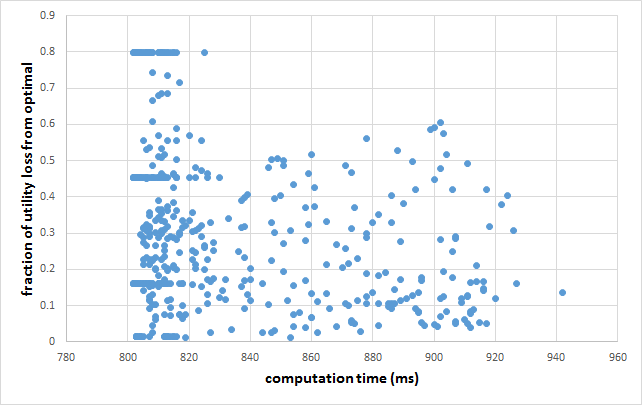
\includegraphics[scale=0.75]{pics/timing-k-2d-sc.eps}
\caption{Relationship between SC approximation computation time and map quality for a two-dimensional knapsack domain.}
\label{fig:timing-k-2d-sc}
\end{center}
\end{figure}


\begin{figure}
\begin{center}
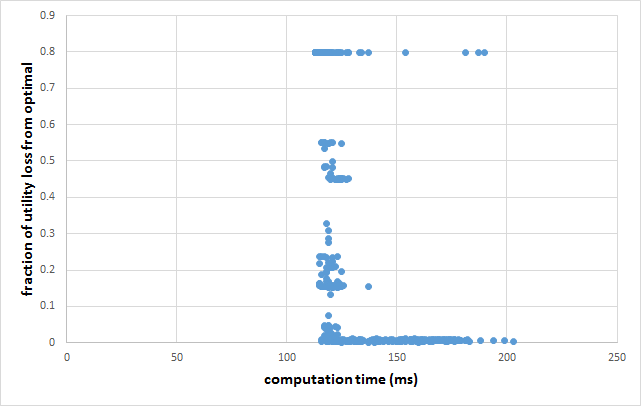
\includegraphics[scale=0.75]{pics/timing-k-2d-al.eps}
\caption{Relationship between SC+AL approximation computation time and map quality for a two-dimensional knapsack domain.}
\label{fig:timing-k-2d-al}
\end{center}
\end{figure}

\begin{figure}
\begin{center}
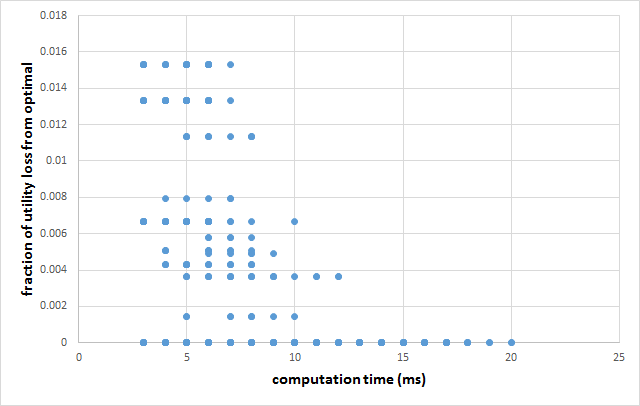
\includegraphics[scale=0.75]{pics/timing-k-2d-sss.eps}
\caption{Relationship between SSS approximation computation time and map quality for a two-dimensional knapsack domain.}
\label{fig:timing-k-2d-sss}
\end{center}
\end{figure}


\begin{figure}
\begin{center}
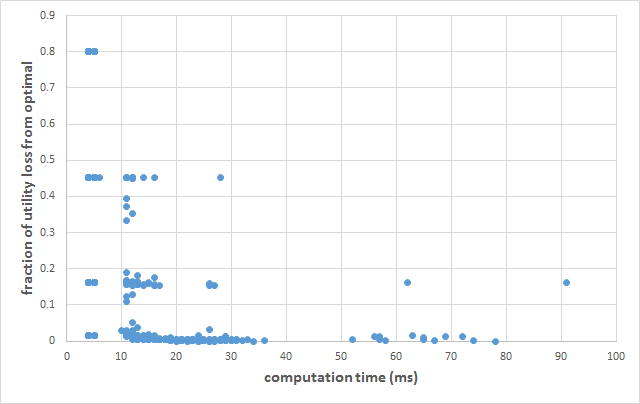
\includegraphics[scale=0.75]{pics/timing-k-2d-svm.eps}
\caption{Relationship between SVM approximation computation time and map quality for a two-dimensional knapsack domain.}
\label{fig:timing-k-2d-svm}
\end{center}
\end{figure}

\begin{figure}
\begin{center}
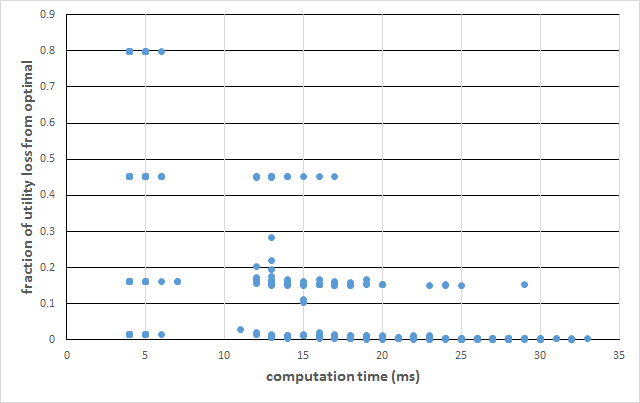
\includegraphics[scale=0.75]{pics/timing-k-2d-svmsbe.eps}
\caption{Relationship between SVM+SBE approximation computation time and map quality for a two-dimensional knapsack domain.}
\label{fig:timing-k-2d-svmsbe}
\end{center}
\end{figure}

Similar to the knapsack problem,  the elevator domain shows a strong correlation between computation time and utility loss when the more sophisticated algorithms are employed, as shown in Figures \ref{fig:timing-elevator6pass-sc} through \ref{fig:timing-elevator6pass-svmsbe}.  However, even the random SC algorithm in this domain seems to show a tendency towards better performance at high sample rates.


It is worth noting the discrete characteristic of several of the maps.  This results from very low variance in utility loss as a function of the discovered solutions.  That is, the set of solutions that the initial sampling discovers tends to determine the overall performance of the approximation algorithm.  This is most evident in the SSS algorithm, in which the assignment of the solutions to unsolved problem instances is most directly determined by the set of discovered solutions.  Recall that in SSS, each unsolved problem is assigned a solution by testing each previously discovered solution.  Other approximation algorithms attempt to avoid testing all discovered  the solutions, but, outside of SC, these algorithms still tend to use the information from the set of discovered solutions in a consistent, although not deterministic, manner.

A similar effect explains the horizontal clustering apparent in several of the maps.  This clustering is a function of low number of solutions in the space, leading to low numbers of permutations of discovered solutions during the initial sampling stage.  Again, the performance of the algorithms is sensitive to the solutions discovered.  Thus the same permutation tends to lead to similar performance of the algorithm, resulting in clustering at a specific utility loss measure.


This discrete characteristic and cluster effect appears less frequently in the elevator domain, likely due to the larger number of solutions available in the domain.  Thus, the set of discovered solutions  is more varied.




\begin{figure}
\begin{center}
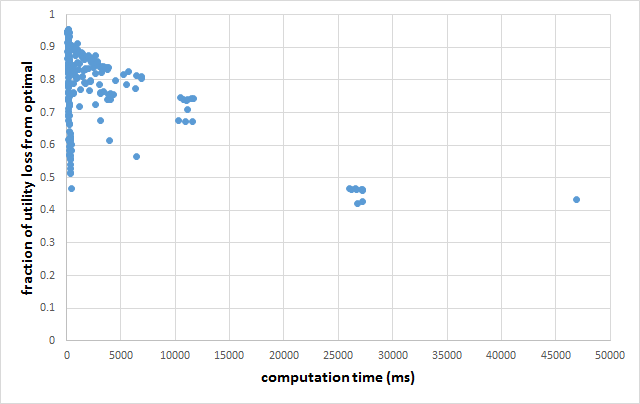
\includegraphics[scale=0.75]{pics/timing-elevator6pass-sc.eps}
\caption{Relationship between SC approximation computation time and map quality for a three-dimensional elevator domain.}
\label{fig:timing-elevator6pass-sc}
\end{center}
\end{figure}

\begin{figure}
\begin{center}
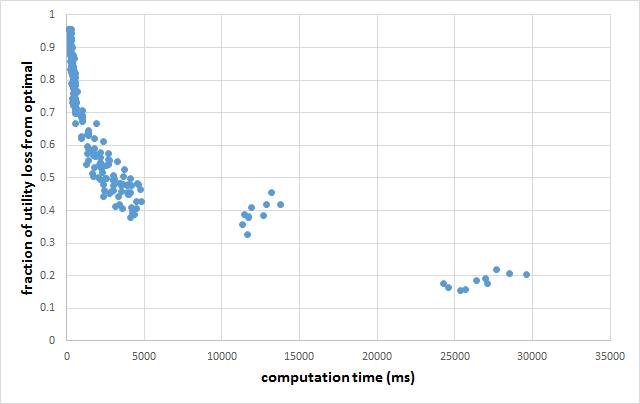
\includegraphics[scale=0.75]{pics/timing-elevator6pass-al.eps}
\caption{Relationship between SC+AL approximation computation time and map quality for a three-dimensional elevator domain.}
\label{fig:timing-elevator6pass-al}
\end{center}
\end{figure}

\begin{figure}
\begin{center}
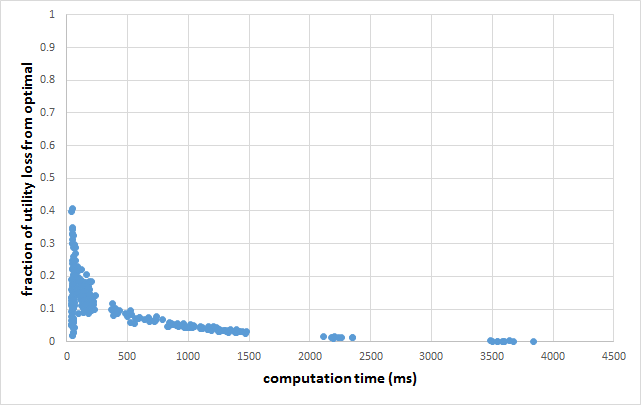
\includegraphics[scale=0.75]{pics/timing-elevator6pass-sss.eps}
\caption{Relationship between SSS approximation computation time and map quality for a three-dimensional elevator domain.}
\label{fig:timing-elevator6pass-sss}
\end{center}
\end{figure}

\begin{figure}
\begin{center}
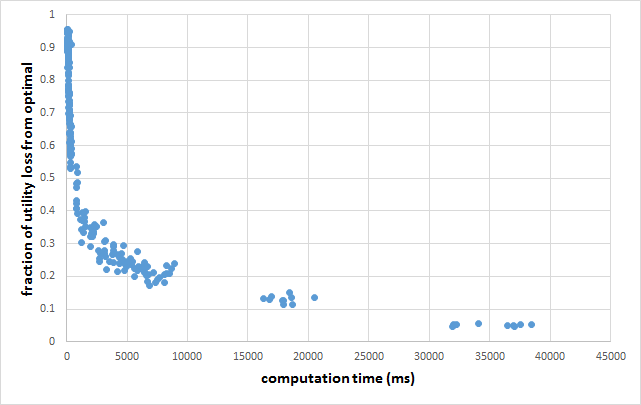
\includegraphics[scale=0.75]{pics/timing-elevator6pass-svm.eps}
\caption{Relationship between SVM approximation computation time and map quality for a three-dimensional elevator domain.}
\label{fig:timing-elevator6pass-svm}
\end{center}
\end{figure}

\begin{figure}
\begin{center}
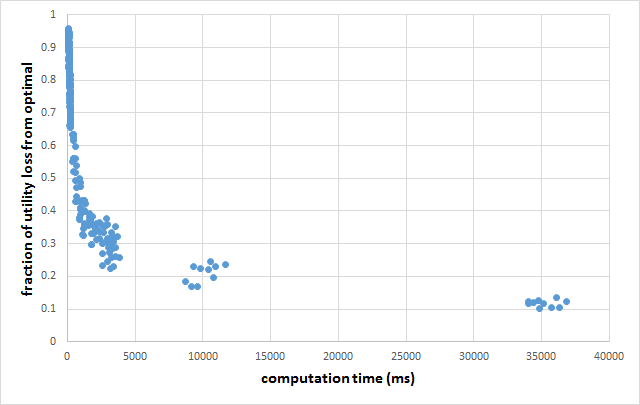
\includegraphics[scale=0.75]{pics/timing-elevator6pass-svmsbe.eps}
\caption{Relationship between SVM+SBE approximation computation time and map quality for a three-dimensional elevator domain.}
\label{fig:timing-elevator6pass-svmsbe}
\end{center}
\end{figure}

%For the elevator domain, I revisit Figure \ref{fig:svmsbe_elevator_12} and assume the best-case online repair fractional utility loss of .065.

This leaves the question of how to accurately estimate the expected performance is for a particular sample rate. Recalling that the effectiveness of the algorithms appears to be a function of the number of size of homogeneous solution regions, it may be possible to estimate the number of homogeneous solution regions by examining the  characteristics of the objective function or the problem configuration.  For example, an elevator domain with configuration M=12, N=6, with one slow elevator per block, has approximately two solution regions:  one in which the elevator in the first block picks up the passenger, and one in which the elevator in the second block picks up the passenger.  One might then speculate that the  number of solution regions is approximately $\frac{M}{N}$, assuming one slow elevator per block and zero fast elevators.  Determining the number of solution regions in other domains is potentially less straightforward.  For example, Figure \ref{fig:five_city_tsps} shows PS Maps for several randomly configured DTSPs.  The unique solutions vary from eight to eleven.


% description of number of unqiue item weights versus number of unique solutions experiment
As one experiment shows, the number of unique solutions in a knapsack PS Map is approximated by the number of unique item weights in the knapsack prior to the consideration of the variable item.  In the first experiment, I started with a knapsack of static items and generated a PS Map for several weight threshold values.  For each weight threshold, I found the knapsack solution and recorded the number of unique item weights.  I then introduced the variable item, generated the PS Map, and recorded the number of unique solutions.

In the second experiment, I kept the weight threshold constant and generated a PS Map for several static item  configurations.  As in the first experiment, I recorded the number of unique weight values in the static item set, added the variable item, generated the PS Map, then recorded the number of unique solutions in the PS Map.

The results of the first experiment demonstrate that the number of unique solutions per number of unique weights is approximately 1.02.




\begin{figure}
\begin{center}
\includegraphics[scale=0.25]{pics/FiveCityFourFixed_0-3.dat.eps}
\caption{Various high-quality PS Maps of five-city TSPs.  Total number of unique solutions varies from eight to eleven.}
\label{fig:five_city_tsps}
\end{center}
\end{figure}


\begin{figure}
\begin{center}
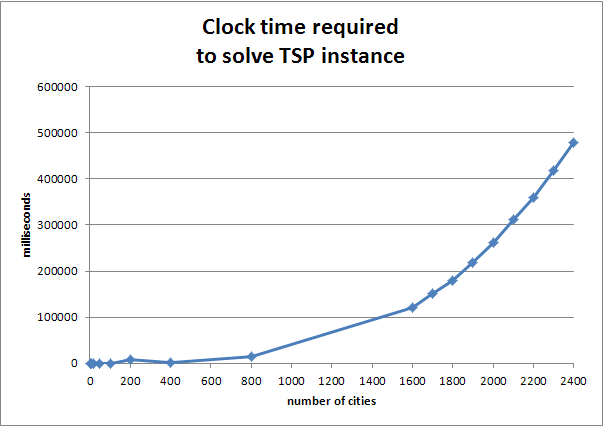
\includegraphics[scale=0.5]{pics/timing-tsp.eps}
\caption{Time required to solve TSP problems of various sizes.  The average time to solve 400-city TSPs is less that required to solve 200-city TSPs.}
\label{fig:timing-tsp}
\end{center}
\end{figure}

\begin{figure}
\begin{center}
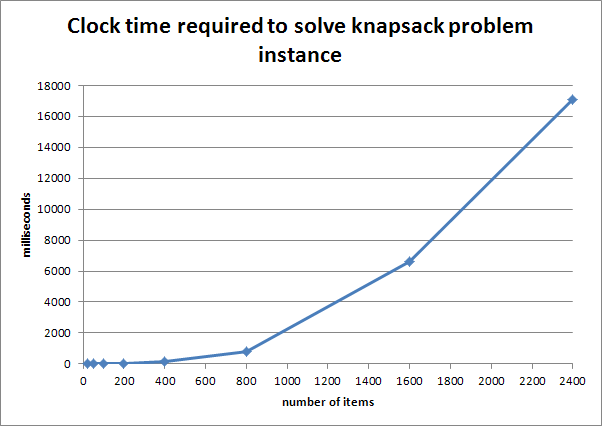
\includegraphics[scale=0.5]{pics/timing-k.eps}
\caption{Time required to solve knapsack problems of various sizes.}
\label{fig:timing-k}
\end{center}
\end{figure}


\section{Scalability of Algorithms}

The time complexity of the algorithms presented is polynomial in the size of the problem space and sample rate, as discussed in Section \ref{sec:complexity} and summarized in Table \ref{tab:summary-of-complexity}.  The overall complexity also depends on the complexity of generating a high-quality solution, which is domain-specific. The largest challenge for algorithm scalability is thus managing the size of the problem space as the problem domains grows in complexity.  Parallelism, as discussed in Section \ref{sec:parallelization}, is a potent mitigation approach.

In the TSP domain, each new location adds two dimensions to the problem space, which quickly increases in size.  As the problem space grows, algorithms that solve large portions of the unsolved problem instances at once, rather than individual problem instances, become more important.  The solution border estimation (SBE) and the support vector machine (SVM) algorithms attempt to find solutions to large regions of the space, and thus could be viable when considering more complex problem domains.  A similar evalution would hold for knapsack problem, in which two dimensions -- one for weight and one for value -- are added to the problem space with every new item that must be considered.  In the elevator domain, each new starting or destination location only adds one dimension to the space, so it grows more slowly.

In terms of space complexity, storing a solution for every problem instance in a simple map would quickly become unwieldy. Initially, moving to a representation such as quad trees, which represent regions of the space, would help.  However, the best solution may be to store models, such as those generated by the SVM and SBE algorithms, rather than mappings from individual problem instances to solutions.  Also the select from sampled solutions (SSS) algorithm could be adapted to only store the solutions it finds and then match a problem instance to a solution at runtime, thereby trading off online reaction time to save storage space.

As the problem size increases, another consideration is the number of samples required to reach a desired level of performance.  Intuitively, it appears that the algorithms' improvement resembles a sigmoid function: as the number of samples increase, the performance slowly improves until the number of samples reaches a critical mass. At that point, performance improve rapidly until the space is effectively represented, making additional samples redundant, and performance levels off. However, I would imagine a high degree of variability due to the stochastic nature of taking samples from a problem space.  For example, if a sample happens upon a key solution, or provides some key information regarding a solution border, then that specific sample could greatly improve the performance of that instance of the algorithm.  Thus it is possible that improvement could vary widely with each sample, particularly in a problem domain in which solutions may have very different utilities.




\chapter{Conclusion \& Future Work}
\thispagestyle{plain}

\label{ch:future}


This dissertation introduced the concept of \textit{plan space analysis} (PSA), specifically the use of Problem-Solution Maps to rapidly allow a system to adjust its plan when it encounters a change in the environment.  Ideally, a system would have a library of plans for numerous possible changes in the environment, thereby being able to select one at runtime, rather than replanning from scratch or engaging in online repair.  Chapter \ref{ch:psa} provided  examples of PS Maps, noted that a brute-force approach to creating a PS Map is not feasible, and presented seven algorithms to approximate a PS Map.  The chapter also presented a complexity analysis of the algorithms.  Chapter \ref{ch:evaluation} described the traveling salesman problem (TSP), knapsack problem, and elevator problem as test domains and presented the results of approximating PS Maps within those domains.  The results demonstrate that the utility of the plans given by the approximated PS Map are frequently comparable to the utility of the plans generated with online repair.  Chapter \ref{ch:application} discussed approaches to determining the tradeoff between using PSA versus online repair, particularly when considering the time available for PSA calculations.  In addition to considering tradeoffs related to timing, the chapter also detailed requirements for representing the problem instances within the problem space.  Namely,
\begin{itemize}
\item The problem space axes should be selected such that problem instances with identical solutions are adjacent.
\item The solutions should be  abstracted in order to create similar solutions, thus allowing for homogeneous solution regions.
\end{itemize}

In the TSP, knapsack, and elevator domains, using the variable features of the problem instance as axes for the problem space was sufficient to create homogeneous solution regions.   However, one could imagine other domains in which there are homogeneous solution regions, but  only with respect to a more complex function of the variable features, such as with the example of the game described in the chapter.  In that case, axes that considered higher-level or derived features, such as whether the numbers rolled on the dice constitute a pair or straight, would be much more useful than axes based on the numbers themselves. 

Abstraction was not required for raw solutions to the TSP and knapsack problems.  However, the elevator domain did require abstraction and canonicalization for the solutions to be appropriate for the algorithms.

Chapter \ref{ch:application} also described the tradeoff between expected performance and offline planning time based on examination of problem characteristics.

 %Consider, for example, a planner plays poker.  It may utilize this framework in order to more quickly determine its actions as function of the cards that it may receive.  Consider that the planner that currently holds AJ and preplans for the next card that it receives.  The resulting plans resulting from the next card being an A or J would likely be similar due to both of those cards creating a pair.  In contrast to our earlier examples, the plans for A and K, although close in vlaue, would not be similar.  In this case a better indexing scheme that considers pair versus non-pair would place A and J close together, likely allowing for the algorithms to perform better by allowing the the indexing to place problem instances with similar solutions adjacent to each other.

Some thoughts for extending this work follow.

\section{Suboptimal Plans}

The PS Map map assists in plan library creation by showing the minimum number of solutions required for optimal competency across the problem space.  In the case of a 5-city DTSP map, as few as only eight solutions are required, representing fewer than 7\% of the 120 (5!) possible solutions.  However, for large problems, storing even 7\% of the possible solutions may not be feasible.  One alternate approach is to accept suboptimal solutions in the library, particularly when one suboptimal plan may replace multiple one or more optimal plans.  In this case, this map gives hints about regions in which tolerating a suboptimal plan over a large region, in place of several plans from smaller regions, may be beneficial in reducing the number of plans in the library.

\section{Automated Plan Abstraction}

%AAAI08-157 Learning Generalized Plans Using Abstract Counting

\cite{srivastava08generalized}'s work describes the process of transforming a plan specific to a single problem instance into a generalized plan that is appliable to more than one problem instance.  This is similar to the transformation done within the elevator domain testing, although \citeauthor{srivastava08generalized} present a general approach in which operation preconditions are examined, thus formalizing the conditions that can be generalized.  This approach would be likely be applicable when applying my work to additional planning domains.  Within the elevator domain, my approach was to transform steps such as 

\begin{verbatim}
move elevator slow0-0 to floor 2
board passenger p1 into elevator slow0-0
\end{verbatim}

\noindent
to 

\begin{verbatim}
elevator slow0-0 picks up passenger p1
\end{verbatim}

\noindent
This allows the plan to be valid for any passenger location within elevator slow0-0's range.  \citeauthor{srivastava08generalized}'s abstractions would include this level of transformation, and might also consider a further generalization such as 

\begin{verbatim}
elevator slow0-0 picks up a passenger within range
\end{verbatim}

\noindent
or even introduce loops such as

\begin{verbatim}
for each passenger p within range
  elevator slow0-0 picks up passenger p
\end{verbatim}

The primary result would be to create similar solutions, for which the appropriate axes could create homogeneous solution regions.  This would also assist with reducing the nuber of plans to store in the library.

\section{Analysis of Problem Configuration and Sample Rate}
As mentioned in Chapter \ref{ch:application}, the ability to estimate the configuration of the solution region would be helpful in determining the appropriate sample rate to increase the effectiveness of the approximation algorithms.  Future work could entail finding a correlation between problem domain configuration and the sample rate that should be targeted for a good approximation.

\section{Sampling-based Motion Planning}
%sampling-based motion planning

In robot motion planning, one way to reduce the computational complexity of path planning is to represent the area of operations as a set of discrete cells and points, called \textit{C-space}.  Sampling the operations area will provide a subset of the obstacles that the plan must have the robot avoid, effectively creating a plan with relaxed constraints.  A plan that is not feasible with the relaxed constraints can be discarded, and plans that are feasible can be further refined.  

The sampling in my algorithms is across full problem instances; the sampling in sampling-based planning is across the constraints of a domain, thus always generating a partially defined problem instance.  This approach would be equivalent to adding an additional index to the solution space that represented the constraint.  Because the obstacles are simply binary -- either the plan will consider the obstacle or it will not -- it may be more efficient to use sampling-based planning to sample the $2^n$ binary combinations rather than adding $n$ additional dimensions.  This would support rapid replanning in cases in which an obstacle appears or disappears during the course of plan execution.

\section{NASA}

\cite{DBLP:conf/aaai/Smith12} describes a challenge that the Mars Rover scientific team faces in which they must decide on a set of goals for a planner to consider.  There are many constraints to consider that would make for a challenging planning problem, however, the key issue is that the scientists do not have a way to evaluate the tradeoffs between the goals they may consider.  \citeauthor{DBLP:conf/aaai/Smith12} proposes a solution in which scientists are able to consider a variety of plans from which they could get a sense of what goal combinations are feasible.  My work could be suitable for this initial need.  However, the second need that \citeauthor{DBLP:conf/aaai/Smith12} describes is plan explanation, in which scientists could ask why one goal is included in the plan and not another, as well as what-if questions that allow them to explore tradeoffs between their goals.  

A PS Map for a planning domain shows the set of solutions available for a set of potential changes in the problem space.  An interesting extension may be a PS Map that gives information about the set of solutions two steps removed from the current environment.  In principle, this could be accomplished by adding axes to the problem space representing all two-hop changes, similar to a TSP PS Map that considers more  than one new location. However, in more traditional planning domain, it may be possible to exploit the temporal relationship between two-hop changes to create the map more efficiently.


%Additionally, \citeauthor{smyth01competence} only address the question of competence in a binary fashion.  One extension of the techniques described in this dissertation would be the Solution-Problem Utility (SPU) Map, which determines the competency of a solution as a measure of utility, thus allowing for tradeoffs to be made after the competency evaluation.  More explicitly, imagine two solutions that both resolve a problem with some utility.  The Solves predicate cannot distinguish between two solutions that are both deemed competent or incompetent, whereas an SPU Map would more finely choose between solutions of varying utility.

%\section{Additional PSA components}

%Although appropriate plan abstraction can reduce the number of plans that must be stored in a library, it may be necessary to further reduce the number of plans.  If the system can plans with less quality, then 

\section{Solver Validation}
In addition to library generation, the SBE techniques suggest a mathematical framework that proves the solution similarity of groups of problem instances.   When comparing approximate maps to the high-quality maps, I found instances of solution variety in regions of the problem space that the SBE technique indicated should be homogeneous.  This led me to develop a ``smoothing'' technique in which I run SSS over specific groups of instances to increase the accuracy of the high-quality maps.   This approach could also be used to compensate for the flaws inherent to a heuristic solver based on search.  Future work could examine confirming the solution of a given problem intance by also solving problem instances that are similar to it and returning the best solution.  How to best mutate the given problem instance to maximize the chance of finding a better solution may be an interesting research question.


\begin{table}
\begin{center}
  \begin{tabular}{|p{4.5cm}|p{3cm}|p{3cm}|}
    \hline
    \textbf{Configuration} & \textbf{Unsmoothed} & \textbf{Smoothed} \\ \hline
    M=24, N=4, 6 slow, 3 fast, 3 variable & 1072 & 506 \\ \hline
    M=24, N=6, 4 slow, 0 fast, 3 variable & 590  & 198 \\ \hline
    \hline
  \end{tabular}
  \caption{Effect on smoothing on PS Maps created by a heuristic solver. ``Configuration'' refers the elevator domain's M and N parameters, the total number of elevators, and the number of passengers with variable starting positions.  ``Unsmoothed'' and ``smoothed'' is the number of unique solutions prior to and after smoothing.}
  \label{tab:smoothing}
\end{center}
\end{table}


\section{Concluding Thoughts}

The challenge of rapidly finding good solutions to complex problems is a theme common to many projects in my workplace.  During the course of this work, I have been happy to discover numerous potential applications for some of the ideas presented here.  I find myself particularly interested in related problems within the Smart Grid and energy management, and hope to explore solutions to problems in that domain.  I hope that the approaches I have developed here may be of some use or inspiration to others encountering these types of problems.

\cleardoublepage
\appendix
%\chapter{Framework}
\thispagestyle{plain}

\label{ch:framework}

The framework adapts to new domains by allowing the specification of the problem instance, solution, and a solver to convert the problem instance into a solution.  Generating PS Maps requires the specfication of a problem space to define the range of problem instances of interest.  Finally, if visualization is desired, a problem space adapter and display augmenter may be defined.

This framework is implemented in Java.  The base classes need to define a problem domain are GenericProblemInstance, GenericSolution, GenericSolver, GenericProblemSpace, ProblemSpaceAdapter, and DisplayAugmenter.

\section{Problem Instance}

A problem instance is defined as set of key-value pairs.  For example, a problem instance in the knapsack domain defines set of items and the knapsack capacity.  Assuming an item is represented as Item(\textit{name},\textit{weight},\textit{value}), a typical key-value pair in the problem instance may be (``map'', Item(``map'',9,150)), where ``map'' is the key, and the item is the value.  The knapsack capacity could be represented by a key-value pair such as (``weight'',400).

In addition to the key-value pairs representing the elements of the problem instance, a definition of distance between problem instances must be defined.  Approximation algorithms that estimate solutions to unsolved problem instances based on the solutions of solved problem instances may use distance to select the solved problem instances to consider.

The abstract GenericProblemInstance class implements the functionality described above.  Users of this class are required to extend the class and define the \textit{distance} method.

\section{Solution}

Similar to a problem instance, a solution is also a set of key-value pairs representing a solution to a problem instance.  In the knapsack problem, this may appear as one key with a value that is a list such as (``items'', (Item(``map'',9,150), Item(``water'',153,200), Item(``umbrella'',73,40)), or one key per item as in the problem instance.

A solution is not specific to a problem instance.  Typically it defines static key-value pairs and may leave open slots for the characteristics of the problem instance to which it is applied.  For example, the solution to a traveling saleman problem is an ordering of coordinate locations with flags to indicate when to visit the location specifed by the problem instance.  One representation may be  ((0,0), (2,0), (3,2), null, (4,4), (6,5)), indicating that when applied to a problem instance, the null element should be replaced with instance's location.  A knapsack solution may not need a specific flag, rather it may define a mapping from an item name to a quantity to be place in the knapsack, thus the solution can be applied to any problem instance that defines item names and their weight and value.

The abstract GenericSolution requires the definition an algorithm for calculating its utility when is it applied to a problem instance.  In addition to a utility calculation, an implementation must also define a function that determines if a solution is feasible for a given problem instance.  In domains such as a traveling salesman problem, this function will always return a true value, as any ordering of locations is feasible.  However a domain with constraints, such as the weight limitation of the knapsack problem, will define this method to enforce those constraints.  Finally, a GenericSolution should define a method to test for equality between solutions.

\section{Solver}

\section{Problem Space}

\section{Visualization}


\cleardoublepage

\thispagestyle{plain}
%\bibliographystyle{aaai}
\bibliographystyle{plainnat}
\bibliography{thesis}

%final blank page per formatting requirements
\newpage
\thispagestyle{empty}
\mbox{}

\end{document}
